% concatenated from GHSW_2026_arXiv.tex
\documentclass[12pt]{article}
\usepackage{amsmath,amssymb,amsthm, amsfonts,xcolor,enumerate}
\usepackage{hyperref,cleveref}
\usepackage{graphicx}
\usepackage{soul}
\usepackage{url}
\usepackage{dsfont} 
\usepackage{color}
\definecolor{red}{rgb}{1,0,0}
\def\red{\color{red}}
\definecolor{blue}{rgb}{0,0,1}
\def\blu{\color{blue}}
\definecolor{green}{rgb}{0,.6,0}
\def\gre{\color{green}}
\definecolor{purp}{rgb}{.5,0,.5}
\def\pur{\color{purp}}
\def\lh#1{\noindent
\textcolor{purp}
{\textsc{(LH:}
\textsf{#1})}}
\def\bls#1{\noindent
\textcolor{green}
{\textsc{(BLS:}
\textsf{#1})}}
\def\hg#1{\noindent
\textcolor{brown}
{\textsc{(HG:}
\textsf{#1})}}
\usepackage{tikz}
\usetikzlibrary{arrows.meta} 
\usepackage{float}


\setlength{\textheight}{8.8in}
\setlength{\textwidth}{6.5in}
\voffset = -14mm
\hoffset = -10mm

\newtheorem{thm}{Theorem}[section]
\newtheorem{cor}[thm]{Corollary}
\newtheorem{lem}[thm]{Lemma}
\newtheorem{prop}[thm]{Proposition}
\newtheorem{conj}[thm]{Conjecture}
\newtheorem{obs}[thm]{Observation}
 \newtheorem{alg}[thm]{Algorithm}
\newtheorem{prob}[thm]{Problem}
\newtheorem{quest}[thm]{Question}

\theoremstyle{definition}
\newtheorem{rem}[thm]{Remark}

\theoremstyle{definition}
\newtheorem{defn}[thm]{Definition}

\theoremstyle{definition}
\newtheorem{ex}[thm]{Example}

\numberwithin{figure}{section}   
\numberwithin{equation}{section}  
\newcommand{\R}{\mathbb{R}}
\newcommand{\C}{\mathbb{C}}

\newcommand{\GL}[1]{\mathcal{G} ^ #1}

\newcommand{\GLG}{G^L}
\newcommand{\GLGsig}{G^{\sigma(L)}}
\newcommand{\GC}[2]{#1 ^ {\mathfrak #2}}
\newcommand{\GAC}[2]{#1 ^ {\mathfrak #2}}

\newcommand{\PP}{\mathfrak{C}}
\newcommand{\pp}{\mathfrak{c}}
\newcommand{\NN}{\mathfrak{N}}
\newcommand{\nn}{\mathfrak{n}}
\newcommand{\MM}{\mathfrak{M}}
\newcommand{\mm}{\mathfrak{m}}
\newcommand{\II}{\mathfrak{I}}
\newcommand{\ii}{\mathfrak{i}}
\newcommand{\Ibb}{\mathbb{I}}

\newcommand{\D}{\Gamma}
\newcommand{\G}{\mathcal{G}}
\newcommand{\F}{\mathcal{F}}
\newcommand{\Span}{\operatorname{span}}
\newcommand{\sym}{\mathcal{S}}
\newcommand{\symp}{\mathcal{S}_+}
\newcommand{\SG}{\mathcal{S}(G)}
\newcommand{\Symp}{\mathcal{S}_+(G)}
\newcommand{\QG}{\mathcal{Q}(\Gamma)}
\newcommand{\K}{{\cal K}}
\newcommand{\Y}{{\cal Y}}
\newcommand{\A}{\mathcal{A}}

\newcommand{\ba}{{\bf a}}
\newcommand{\bb}{{\bf b}}
\newcommand{\bc}{{\bf c}}
\newcommand{\be}{{\bf e}}
\newcommand{\bz}{{\bf z}}
\newcommand{\by}{{\bf y}}
\newcommand{\bx}{{\bf x}}
\newcommand{\bv}{{\bf v}}
\newcommand{\bw}{{\bf w}}
\newcommand{\bu}{{\bf u}}

\newcommand{\symm}{\operatorname{Symm}}
\newcommand{\Sp}{\operatorname{Sp}}
\newcommand{\spLA}{\operatorname{\mathfrak{sp}}}
\newcommand{\Mp}{\operatorname{M}_+}
\newcommand{\adj}{\operatorname{Adj}}
\newcommand{\oml}{{\bf m}}
\newcommand{\soml}{{\bf m}_s}
\newcommand{\tp}{\operatorname{TP}}
\newcommand{\Rnn}{\R^{n\times n}} 
\newcommand{\Rpp}{\R^{p\times p}} 
\newcommand{\Rn}{\R^{n}} 
\newcommand{\Znn}{\Z^{n\times n}} 
\newcommand{\Zn}{\Z^{n}} 
\newcommand{\Fnn}{F^{n\times n}} 
\newcommand{\Fmn}{F^{m\times n}} 
\newcommand{\Fn}{F^{n}} 

\newcommand{\trans}{^{\top}}
\newcommand{\tr}{\operatorname{tr}}
\newcommand{\perps}{^{\perp}|_{\symm}}

\newcommand{\Z}{\operatorname{Z}}
\newcommand{\ZC}{\Z_{\operatorname{C}}}
\newcommand{\Zell}{\Z_{\ell}}
\newcommand{\M}{\operatorname{M}}
\newcommand{\MC}{\M_{\operatorname{Sp}}}
\newcommand{\dist}{\operatorname{dist}}
\newcommand{\im}{\operatorname{Im}}


\newcommand{\mtx}[1]{\begin{bmatrix} #1 \end{bmatrix}}


\newcommand{\spec}{\operatorname{spec}}
\newcommand{\range}{\operatorname{range}}
\newcommand{\nul}{\operatorname{null}}
\newcommand{\Gc}{\overline{G}}
\newcommand{\diag}{\operatorname{Diag}}
\newcommand{\spspec}{\operatorname{SPspec}}
\newcommand{\uvec}{\operatorname{vec}_\triangle}


\newcommand{\n}{\{1,\dots,n \}}
\newcommand{\noi}{\noindent}
\newcommand{\x}{\times}
\newcommand{\lam}{\lambda}
\newcommand{\Lam}{\Lambda}
\newcommand{\LS}{\Lambda^S}
\newcommand{\bit}{\begin{itemize}}
\newcommand{\eit}{\end{itemize}}
\newcommand{\ben}{\begin{enumerate}}
\newcommand{\een}{\end{enumerate}}
\newcommand{\beq}{\begin{equation}}
\newcommand{\eeq}{\end{equation}}
\newcommand{\bea}{\begin{eqnarray*}}
\newcommand{\eea}{\end{eqnarray*}}
\newcommand{\bean}{\begin{eqnarray}}
\newcommand{\eean}{\end{eqnarray}}
\newcommand{\bpf}{\begin{proof}}
\newcommand{\epf}{\end{proof}\ms}
\newcommand{\bmt}{\begin{bmatrix}}
\newcommand{\emt}{\end{bmatrix}}
\newcommand{\ms}{\medskip}
\newcommand{\noin}{\noindent}
\newcommand{\beqa}{\begin{array}}
\newcommand{\eeqa}{\end{array}}
\newcommand{\OL}{\overline}
\newcommand{\lc}{\left\lceil}
\newcommand{\rc}{\right\rceil}
\newcommand{\lf}{\left\lfloor}
\newcommand{\rf}{\right\rfloor}
\newcommand{\lp}{\left(}
\newcommand{\rp}{\right)}
\newcommand{\lb}{\left[}
\newcommand{\rb}{\right]}
\newcommand{\lsb}{\left\{}
\newcommand{\rsb}{\right\}}
\newcommand{\wt}{\widetilde}
\newcommand{\wh}{\widehat}
\newcommand{\cp}{\mathbin{\Box}}
\newcommand{\du}{\mathbin{\,\sqcup\,}}


\newcommand{\dub}{D^{(2)}}


\def\tw#1{\noindent
\textcolor{teal}
{\textsc{(TW:}
\textsf{#1})}}

\title{The Inverse Symplectic Eigenvalue Problem of a Graph}
\author{Himanshu Gupta\thanks{Department of Mathematics and Statistics, University of Regina, Regina, SK S4S0A2, Canada (himanshu.gupta@uregina.ca)} \and Leslie Hogben\thanks{American Institute of Mathematics, Pasadena, CA 91125, USA
(hogben@aimath.org); Department of Mathematics, Iowa State University,
Ames, IA 50011, USA; Department of Mathematics, Purdue University,
West Lafayette, IN 47907, USA.}\and Bryan Shader\thanks{Department of Mathematics \& Statistics, University of Wyoming, Laramie, WY 82071, USA (bshader@uwyo.edu)}\and Tony Wong\thanks{Department of Mathematics, Kutztown University of Pennsylvania, Kutztown, PA 19530, USA (wong@kutztown.edu)}}




\begin{document}
\maketitle

\begin{abstract} 
Symplectic geometry plays an increasingly important role in mathematics, physics and applications, and naturally gives rise to interesting matrix families and properties. One of these is the notion 
of symplectic eigenvalues, whose existence for positive definite matrices is known as Williamson's theorem or decomposition.  This notion of symplectic eigenvalues 
gives rise to inverse problems. 
We introduce the inverse symplectic eigenvalue problem for positive definite matrices described by a labeled graph and  solve it for several families of labeled graphs and all labeled graphs of order  four.  To solve these problems we develop various tools such as the Strong Symplectic Spectral Property (SSSP) and its consequences such as the Supergraph Theorem, the Bifurcation Theorem, and the Matrix Liberation Lemma for symplectic eigenvalues, graph couplings to describe collections of labelings of a graph that produce the same symplectic eigenvalues, and coupled graph zero forcing.  We establish numerous results for symplectic positive definite matrices, including a sharp lower bound on the number of nonzero entries of such a matrix (or equivalently, the number of edges in its graph).  This lower bound is a consequence of a  lower bound on the sum of number of nonzero entries in an  irreducible positive definite matrix and its inverse. 


\end{abstract}


\noi {\bf Keywords} symplectic matrices, symplectic eigenvalues of positive definite matrices, inverse problems, strong properties, zero forcing, graphs. 

\noi{\bf AMS subject classification} 15A18, 15B48, 15B57, 05C50. 

 
%%%%%%%%%%%%%%%%%%%%%%%%%%%%%%%%%%%%%%%%%%%








\section{Introduction}\label{s:intro} 
Let 
\[ 
\Omega_{n} = \left[ \begin{array}{rc} O_p & I_p \\ 
-I_p &O_p \end{array} \right],\]
where $n=2p$ and  $I_p$ (respectively, $O_p$) denotes the $p\times p$
identity (respectively, zero) matrix; when the order is clear from context, we may omit the subscript.  
The {\it symplectic group of order $n$} is denoted by $\Sp(n)$
and is the set of all $n \x n$ real matrices $S$ such that $
S\trans \Omega S=\Omega$.
Evidently, the symplectic matrices of order $n$
are those block matrices  of the form 
\[
\left[ 
\begin{array}{rc} 
S_{11} & S_{12} \\  
S_{21} & S_{22} \end{array}
\right], 
\]
where each block is $p\x p$, $S_{11}\trans S_{21}$ and $S_{12}\trans S_{22}$ are symmetric, and $S_{11}\trans S_{22}-S_{21}\trans S_{12}=I$. 
Examples of symplectic matrices  include
\begin{align}
\label{basic}
\mbox{ $\Omega, \quad \mtx{A & O\\O & (A^\top)^{-1}}$, \quad  and \quad  $\mtx{I & B\\O & I}$},
\end{align}
where $A$ and $B$ are $p \times p$ real matrices, $A$ is invertible, and $B$ is symmetric; the matrices in \eqref{basic} are called \emph{basic symplectic matrices}. 
The $n\times n$ symplectic matrices are closed under products, inverses, and transposes. It is known that 
every $n\times n$ symplectic matrix $S$ is a finite product of matrices  of the forms in \eqref{basic}. Indeed, {it is shown in} \cite{JLX22} 
 that  $S$ is a product of at most five basic symplectic matrices of the third type and/or their transposes.



Symplectic matrices arise geometrically and can be viewed as an analog of real orthogonal matrices:  The standard Euclidean space of dimension $m$ consists of $\mathbb{R}^m$ endowed with 
the bilinear form $\langle \bx, \by\rangle= \bx^\top I \by= \bx^\top \by$. An $m\times m$ orthogonal matrix
$Q$ is precisely a matrix that preserves this bilinear form (that is, 
$\langle Q\bx, Q\by\rangle= \langle \bx, \by \rangle$ for all $\bx, \by \in \mathbb{R}^m$).
The  standard \textit{symplectic vector space of dimension $n=2p$} consists of $\Rn$  endowed with  the bilinear form  $\langle\langle \bx , \by \rangle\rangle= \bx^\top\Omega \by$.  The matrix $S$ is symplectic if and only if 
$\langle\langle S\bx, S \by \rangle\rangle= \langle\langle \bx, \by \rangle\rangle$ for all $\bx, \by \in \mathbb{R}^{n}$; that is, if and only if 
the map $\bx \mapsto S\bx$ preserves the bilinear form $\langle\langle \, , \, \rangle \rangle$.
In short, symplectic matrices are to symplectic spaces as orthogonal matrices are to Euclidean spaces. 



The classic spectral theorem for real symmetric matrices asserts that each symmetric matrix $A$ is 
orthogonally similar to a diagonal matrix whose entries are the eigenvalues of $A$.
{The analog of this result in the symplectic setting is based on Williamson's  work on matrix pencils \cite{W36} applied to 
real positive definite matrices, which by definition are symmetric. 
For an elementary proof of Williamson's Theorem, see \cite{I18}.}

\begin{thm}[Williamson's Theorem]
Let $N$ be an $n \times n$ real positive definite matrix with $n=2p$. 
Then there exists a symplectic matrix $S$ and a $p\times p$ diagonal matrix $D$ such that 
\[ S\trans N S= \left[ \begin{array}{cc}
D & O \\
O & D \end{array} \right] .\]
Moreover, the diagonal entries  of $D$ are unique {up to re-ordering}.
\end{thm}
The $p$ diagonal entries of the diagonal matrix $D$ in Williamson's Theorem  are called the {\it symplectic eigenvalues of $N$}; the multiset of $p$ symplectic eigenvalues of $N$ is called the \emph{symplectic spectrum of $N$} and is denoted by $\spspec(N)$.
Since $S\trans NS$ is congruent to $N$, and $N$ is positive definite, each symplectic eigenvalue 
is positive.  The \textit{multiplicity} of the symplectic eigenvalue $\lambda$ of $N$
is defined to be the number of occurrences of $\lambda$ on the diagonal of $D$. A symplectic eigenvalue is \textit{simple}
if its multiplicity is one. 

Recent research on the symplectic eigenvalues of positive definite matrices includes
(a) study of basic mathematical properties \cite{Dopico-Johnson},
(b) extension of classical eigenvalue inequalities to the symplectic setting \cite{BJ15,J21,P22,SS22}, 
(c) numerical algorithms for calculating the symplectic eigenvalues \cite{SABT21}, and 
(d) their central roles in understanding  oscillations in the Hamiltonian dynamics setting, 
quantum entanglement and information, and optics (see \cite{N21} and 
references therein).

The next result is a well-known method for theoretically calculating symplectic eigenvalues that suits our purposes. 
\begin{prop}
\label{sympev}
Let $N$ be an $n\times n$ real positive definite matrix with $n=2p$.
Then 
\ben[$(a)$]
    \item 
    \label{sympev-a}
    Each eigenvalue of $\Omega N$ is purely imaginary and nonzero.
    \item
     \label{sympev-b}
    The moduli of the eigenvalues of $\Omega N$ are the symplectic eigenvalues of $N$.
    \item  
    \label{sympev-c}
    The multiplicity of $\lambda$ as a symplectic eigenvalue of $N$ is half the number 
     of eigenvalues of $\Omega N$ having moduli  $\lambda$. This also equals the dimension of the nullspace of 
     $\Omega N-\lambda \sqrt{-1} I$.
\een 
\end{prop}
\begin{proof}
By Williamson's Theorem, there exists an $n\times n$ symplectic matrix $S$
such that $S\trans N S= D \oplus D$, where $D=\diag(d_1, \ldots,d_p)$  whose diagonal entries are the 
symplectic eigenvalues of $N$. Since $S$ is symplectic, 
so is $S\trans$.  Thus, $S \Omega S\trans=\Omega$ and  $\Omega N= S\Omega(D\oplus D) S^{-1}$.  Hence $\Omega N$
is similar to 
\[ 
\Omega (D\oplus D)= \mtx {\begin{array}{rc} O & D \\  -D & O 
\end{array} },
\]
whose eigenvalues are $\pm d_j\sqrt{-1} $ for $j=1,\ldots, p$.
Statements \eqref{sympev-a}--\eqref{sympev-c} readily follow.  
\end{proof}

We use the notation $\spec(A)$ to denote the (standard) spectrum of a square matrix $A$.

 \begin{ex}
\label{ex:directsum}
Let $A$ and $B$ be $p\times p$ positive definite matrices, and 
$N=A\oplus B$.   
Since $(\Omega N)^2=\mtx{-BA & O\\O & -AB}$ and $\spec(AB)=\spec(BA)$, the 
(standard) eigenvalues of $\Omega N$ are the square roots of the (standard) eigenvalues of $-AB$.
If we take $B=A^{-1}$, then $AB=I$ and the symplectic eigenvalues of $A \oplus B$ are all equal to one. If we take $B=A$, then $AB=A^2$ and the symplectic eigenvalues of $A \oplus A$ are the (standard) eigenvalues of $A$. 
\end{ex}


The set $\{Q\trans Q\colon Q \text{ is orthogonal}\}$ is equal to $\{I\}$. The analogous set in the symplectic setting  $\{S\trans S\colon S \text{ is symplectic}\}$ is richer, in terms of both matrices and graphs.  Williamson's Theorem implies that 
every matrix of the form $S\trans S$ with $S$  symplectic has each of its symplectic eigenvalues equal to one,  
while the identity matrix
$I$ is the  
only $n\times n$ symmetric matrix having each eigenvalue equal to one.
For the orthogonal case the corresponding graph is just the empty graph. However, for the symplectic case there are many non-trivial graphs. 
In particular, one is the only symplectic eigenvalue of the $n \times n$ matrix 
\begin{align}
\label{spec_arb_ex}
\mtx{ I & J \\
      O & I
}^\top \mtx{ I & J \\
     O & I}
      = \mtx{I & J \\ J &  pJ+I},
\end{align}
 where $J$ is the all ones matrix (see Example \ref{pK1veeKp} for further discussion).  In Section \ref{s:PD}, we list  several equivalent characterizations of $n\times n$ positive definite matrices that have a single eigenvalue (of multiplicity $p$), give several other  examples of such matrices, and establish some results on the sparsity of such matrices. 

In the setting of spectra of real symmetric matrices, there is a rich body of work on the relationship 
between the spectra and the associated graph of the matrix. In  this work 
we initiate the study of the analogous 
relationship in the symplectic setting. The next definitions allow us to make this more precise. 
 These will seem unduly formal to those familiar with the IEP-$G$, since as we will see, the  labeling of the graph does not affect the (standard) eigenvalues.  However, the corresponding symplectic problem is more subtle: while many relabelings preserve the symplectic eigenvalues, not all do. 
 
 Throughout this paper,  the term \emph{graph} means {an unlabeled,} simple, undirected, and finite graph (with nonempty vertex set), whereas the term \emph{digraph} means {an unlabeled} directed graph.
 A \emph{labeled graph} $G^L$ of order $n$ has a vertex set $V(G^L)=\{1,\dots,n\}$ and  an edge set $E(G^L)$ that is a set of two element subsets of vertices. For such a labeled graph $G^L$,   $\sym(\GLG)$   denotes the set of all symmetric  matrices $A=[a_{ij}]$ 
 where for $i\ne j$, $a_{ij}\neq 0$ if and only if   $ij$ is an edge of $G^L$; in the literature, the labeling is suppressed and this is denoted by $\sym(G)$. 
 For a permutation $\sigma$ of $1,\ldots, n$,  the labeled graph obtained from $G^L$ by re-labeling 
the vertex labeled $i$ by the label $\sigma(i)$ is  denoted by $\GLGsig$. Let $P_{\sigma}$ be the permutation matrix corresponding to $\sigma$, i.e., the matrix obtained from $I$ by placing column $\sigma(i)$ of $I$ in column $i$ of $P_{\sigma}$ .
Then the  matrices $A$ and $P_\sigma AP_\sigma^\top$ are permutationally similar, and 
$A \in  \sym(\GLG)$ if and only if $P{_\sigma} A P_\sigma^\top \in  \sym(\GLGsig)$.
 Thus, the inverse eigenvalue problem for $\sym(\GLG)$ and $\sym(\GLGsig)$
are the same. That is, for  the IEP-$G$,  the labeling of the vertices of $G$ is immaterial, so it is reasonable to suppress the labeling in the notation. 

For symplectic eigenvalues, there is more subtlety.  Unlike the (standard) eigenvalue case, there are constraints on the permutation $\sigma$ that are needed to guarantee the symplectic eigenvalues are preserved. 
That is, not all permutation similarities preserve symplectic eigenvalues. 
\begin{ex}
 Consider
\[ 
N= \left[\begin{array}{rrrr}
2 & 0 & 1 & 1 \\
0 & 2 & 1 & 0 \\
1 & 1 & 2 & 0 \\
1 & 0 & 0 & 2
\end{array}\right]\] 
and $\sigma=(1\, 2\, 4)$.
Then 
\[ 
P_{\sigma} = \left[ \begin{array}{cccc}
0 & 0 & 0 & 1\\
1& 0 & 0 & 0\\
0 & 0 & 1 & 0\\
0& 1 & 0 & 0 
\end{array} 
\right] ,
\quad \mbox{ and } \quad 
 P_\sigma NP_\sigma^\top=
\left[\begin{array}{rrrr}
2 & 1 & 0 & 0 \\
1 & 2 & 1 & 0 \\
0 & 1 & 2 & 1 \\
0 & 0 & 1 & 2
\end{array}\right] .
\] 
The (approximate)  symplectic spectra  of $N$ and $ P_\sigma NP_\sigma^\top$ are  $\{ 1.902, 1.176\}$  and $\{3.078, {0.727}\}$,
respectively  (recall these can be computed as in Proposition \ref{sympev}).  
The example above, which is illustrated in Figure \ref{fig:1}, shows that the symplectic eigenvalues for these two labelings of the path on four vertices  need to be handled separately. 



\begin{figure}[H]
\begin{center}
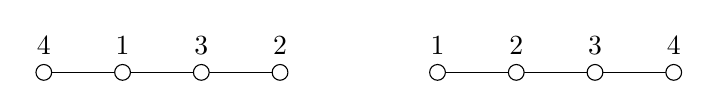
\begin{tikzpicture}
    \draw(1,0)--(4,0);\foreach\i in{1,2,3,4}{\draw[fill=white](\i,0)circle(0.1);};
    \node[above]at(1,0.1){$4$};\node[above]at(2,0.1){$1$};\node[above]at(3,0.1){$3$};\node[above]at(4,0.1){$2$};

    \draw(6,0)--(9,0);\foreach\i in{1,2,3,4}{\draw[fill=white](\i+5,0)circle(0.1);};
    \node[above]at(6,0.1){$1$};\node[above]at(7,0.1){$2$};\node[above]at(8,0.1){$3$};\node[above]at(9,0.1){$4$};
 \end{tikzpicture}
  \caption{Two labelings $L$ and $\sigma(L)$ of $P_4$ where the matrices $N\in \symp(P_4^L)$ and $P_\sigma NP_{\sigma}\trans\in \symp(P_4^{\sigma(L)})$ have different symplectic eigenvalues. 
 \label{fig:1}}
 \end{center}
\end{figure}
\end{ex}
Thus, it is imperative when discussing 
symplectic eigenvalues of matrices associated with a labeled graph $G^L$ that the vertex labels of $G^L$ be taken into consideration. 
  Given a labeled graph $G^L$, we will use $\symp(\GLG)$ to denote the set of  positive definite matrices  $N=[n_{ij}]$   where $n_{ij}\neq 0$ if and only if  $i=j$ or  $ij$ is an edge of $G^L$ (note when studying the IEP-$G$,  $\Symp$ is commonly used to denote the analogous set of positive semidefinite matrices).







 Given an $n\x n$ positive definite matrix $N$, it is  useful to talk about the \emph{labeled graph of $N=[n_{ij}]$}, denoted by $\GL L(N)$, which has vertices $1,\dots,n$ and edge set $\{ij\colon n_{ij}\neq 0$ and  $i\ne j\}$.   


We are now able to begin studying  spectral problems related to  $\symp(G^L)$, where $G^L$ is a labeled graph on $n=2p$ vertices, such as:
\ben[(a)]
\item\label{item-a} Which multi-sets of $p$ positive real numbers are the symplectic spectra of  {matrices} in  $\symp(G^L)$?
 \item\label{item-d} Which {ordered} partitions  of $p$ can be realized as  the {ordered} lists of  multiplicities of symplectic eigenvalues of {matrices} in  $\symp(G^L)$?
\item\label{item-b} What is the largest multiplicity of a symplectic eigenvalue among the matrices in  $\symp(G^L)$?
\item\label{item-dx}  
Which labeled graphs allow a positive definite matrix having only one symplectic eigenvalue?
\een

 Questions \eqref{item-a}, \eqref{item-d}, and \eqref{item-b} are the analogs of the  well-studied inverse eigenvalue problem, inverse multiplicity problem, and maximum multiplicity problem; 
we call these the \textit{inverse symplectic eigenvalue problem for labeled graphs} (the ISEP-$G$, for short), the \emph{inverse symplectic multiplicity problem for labeled graphs}, and the \emph{maximum symplectic  multiplicity problem for labeled graphs}. 
Question  \eqref{item-dx} can be thought of as the symplectic analog of the study of graphs that allow a symmetric matrix having only two distinct eigenvalues.  As noted in \cite{F+13}, such a graph allows an orthogonal symmetric matrix, and as shown in Section \ref{s:PD}, a graph that allows a positive definite matrix having only one symplectic eigenvalue allows a symplectic positive definite matrix.
The rest of this paper  is devoted to studying various aspects of these problems.  

In Section \ref{s:order4} we give a complete resolution of the ISEP-$G$ for all labeled graphs of order four by applying the
theory developed in Section \ref{s:strong}
 and developing additional tools for solving the ISEP-$G$.  
Empty graphs (those with no edges and denoted by $\OL{K_n}$)
are the only graphs for which each multi-set of real numbers is the spectrum of some $ A \in \SG $.
 However, there are many examples of labeled graphs $G^L$ on $n=2p$ vertices such that 
every multi-set of $p$ positive real numbers is the symplectic spectrum of some $N\in\symp(G^L)$. 
We call such  
labeled graphs \textit{symplectic spectrally arbitrary} and study such  graphs in Section \ref{s:ssa}.  Necessarily, if $G^L$ is a  symplectic spectrally arbitrary labeled graph, then  $\symp(G^L)$ contains a matrix with just one symplectic eigenvalue, and hence results in  Section \ref{s:PD} are useful in Section \ref{s:ssa}. 


In the IEP-$G$ there are various conditions (e.g., the Strong Arnol'd Property, the Strong Spectral Property, 
the Strong Multiplicity Property) that have proven to be very useful.  In Section \ref{s:strong} we introduce 
the symplectic analog of the Strong Spectral Property, called the Strong Symplectic Spectral Property or SSSP, state several useful theorems (the Supergraph Theorem, the Bifurcation Theorem, the Matrix Liberation Lemma), and  illustrate how to use these theorems
to establish several results about the ISEP-$G$ { (some of the proofs that are similar to those for the IEP-$G$ are deferred to Appendix \ref{appendix}). In particular, in Section \ref{s:strong} we resolve the  inverse symplectic multiplicity problem  for any labeled graph  $G^L$ such that there is a matrix $\symp(G^L)$ that has only one symplectic eigenvalue and  has the SSSP. 

In Section \ref{s:zeroforcing}, we introduce a new type of zero forcing (coupled zero forcing) and show that  the coupled zero forcing number is an upper bound for maximum symplectic multiplicity.  We also characterize all graphs with coupled zero forcing number equal to one and solve the ISEP-$G$ for several additional labeled graph families.} 
We conclude in Section \ref{s:conclude} with a summary of the labeled graphs for which we have solved the ISEP-$G$ and the tools used to solve them. 
 
 

\ms



The remainder of this section contains some standard notation and terminology. We use $|\mu|$  to denote the modulus (also known as the magnitude or absolute value) of the complex number $\mu$. 

For an $m\times n$ matrix 
$A$, $\alpha \subseteq \{1,\ldots, m\}$ and $\beta\subseteq\{1,\ldots n\}$,  we define the  $A[\alpha, \beta]$ (respectively, $A(\alpha, \beta)$) to be the submatrix of $A$ obtained by keeping (respectively, deleting) 
those rows in $\alpha$ and those columns in $\beta$.
When $A$ is square, we abbreviate 
$A[\alpha,\alpha]$ to $A[\alpha]$, and $A(\alpha, \alpha)$ to $A(\alpha)$.
An $n\times n$ matrix $A$  is \textit{reducible} provided there is a permutation matrix $P$ such that 
$PAP^\top$ has the block matrix form 
\[
\begin{bmatrix}
A_{11} & A_{12}
\\
O & A_{22}
\end{bmatrix},
\]
where 
$A_{11}$ and $A_{22}$ are square, non-vacuous matrices. 
A matrix is \textit{irreducible} if it is not reducible  (in particular, each $1\times 1$ matrix is irreducible). 





 A (simple,  undirected) graph $G=(V(G),E(G))$ has a finite nonempty set of vertices $V(G)$ and a set of edges $E(G)$ where each edge is a two-element set of vertices; edge $\{u,v\}$ is usually denoted by $uv$.  
 A graph $G$ is a \emph{subgraph} of a graph $H$ if $V(G)\subseteq V(H)$ and $E(G)\subseteq E(H)$; in this case, we also say that $H$ is a \emph{supergraph} of  {$G$}.  For $U\subseteq V(G)$, the \emph{subgraph  of $G$ induced by $U$}, denoted by $G[U]$, is the subgraph of $G$ with $V(G[U])=U$ and $E(G[U])=\{uv\colon uv \in E(G) \mbox{ and } u,v\in U\}$; $G[U]$ is also called an 
\emph{induced subgraph} of $G$. 
The \emph{complement} of $G$, denoted by $\OL{G}$, is the graph having vertex set $V(G)$ and edge set that includes edge $uv$ if and only if $uv\not\in E(G)$. 
The \emph{union} of graphs $G$ and $G'$, denoted by  $G\,\cup\, G'$, is the graph with $V(G\cup G')=V(G)\cup V(G')$ and $E(G\cup G')=E(G)\cup E(G')$; if $V(G)\cap V(G')=\emptyset$, this is a \emph{disjoint union} of graphs and is denoted by $G\du G'$. If $V(G)$ and $V(G')$ are disjoint, the \emph{join} of $G$ and $G'$, denoted by $G\vee G'$,  is the graph obtained from $G\du  G'$ by adding all possible edges between $V(G)$ and $V(G')$.  
 
Vertices $u,v\in V(G)$ are \emph{adjacent}  if $uv\in E(G)$. 
The (open) \emph{neighborhood} of a vertex $v$ is $N_G(v)=\{u\in V(G)\colon uv\in E(G)\}$, and the \emph{closed neighborhood} is $N_G[v]=N_G(v)\cup\{v\}$; when $G$ is clear from the context, the subscript may be omitted.  The \emph{degree}  of a vertex $v\in V(G)$ is $\deg_G(v)=|N_G(v)|$. 
A vertex of degree one is called a \emph{leaf}. The minimum degree among the vertices of the graph $G$ is denoted by $\delta(G)$.   A \emph{matching} in a graph $G$ with $V(G)=\{v_1,\dots,v_n\}$ is a set  $\{v_{i_1}v_{j_1},\dots, v_{i_k}v_{j_k}\}\subseteq E(G)$ such that  all the vertices $v_{i_s}, v_{j_t}, s,t=1,\dots,k$ are distinct. A \emph{perfect matching} in  $G$ is a matching that includes all vertices of $G$.
 
 
 A \emph{digraph} $\Gamma=(V(\Gamma),E(\Gamma))$ is a simple directed graph. The  set of vertices $V(\Gamma)$ is finite  and nonempty. An \emph{arc} is an ordered pair of vertices and $E(\Gamma)$ denotes the set of arcs of $\Gamma$, so \emph{loops} (arcs of the form $(v,v)$) and both the arcs $(u,v)$ and $(v,u)$ are allowed, but duplicate arcs are not allowed.  
 A digraph $\Gamma$ is 
\textit{strongly connected}
provided for each ordered pair of vertices $(u,v)$ of $\Gamma$ there is a directed walk in $\Gamma$ from $u$ to $v$. The adjacencey matrix $\A_\Gamma$ of $A=[a_{ij}]\in\Rnn$ has $V(\Gamma)=\{1,\dots,n\}$ and $(i,j)\in E(\Gamma)$ if and only if $a_{ij}\ne 0$.
Thus, $\Gamma$ is strongly connected if and only if  the  adjacency matrix of $\Gamma$ is irreducible. The \textit{strong components} of $\Gamma$ are the maximal induced {strongly connected} subdigraphs of $\Gamma$. 
The vertex sets $V_1$, $\ldots, V_k$ of the strong components partition the vertices of $\Gamma$ and can be ordered so that if $(u,v)$ is an arc of $\Gamma$
with $u\in V_i$ and $v \in V_j$, then $i\leq j$. Given an $n\x n$ positive definite matrix $N$ with $n=2p$ of the form $\mtx{A & B\\B\trans & C}$ with each block $p\times p$, it is also sometimes useful to talk about the \emph{labeled digraph of $B=[b_{ij}]$}, denoted by $\Gamma^L (B)$, which has vertices $1,\dots,p$ and arc set $\{(i,j): b_{ij}\neq 0
\}$.

Graphs $G$ and $H$ are 
isomorphic, denoted $G \cong H$ provided there is a bijection $\phi$ between the vertex set of $G$ and the vertex set of $H$ such that $u$ and $v$ are adjacent in $G$ if and only if $\phi(u)$ and $\phi(v)$ are adjacent in $H$.  The notion of isomorphic digraphs is defined similarly. 
 
%%%%%%%%%%%%%%%%%%%%%%%%%%%%%%%%%%%%%%%%%%%

\section{Symplectic positive definite 
matrices}\label{s:PD}


We begin the study of the ISEP-$G$ with a problem whose analog for the IEP-$G$ has a very simple resolution,  but for the ISEP-$G$ is much more complex.  An $n\times n$ symmetric matrix  $A$ that has   only one eigenvalue is a scalar matrix, and hence its graph  $\G(A)\cong \OL{K_n}$ is disconnected if $n>1$. 
However, in the symplectic setting the situation is very different, as we saw that the matrix in Equation (\ref{spec_arb_ex}) is both symplectic and positive definite, and has exactly one symplectic eigenvalue.

 If $N$ is positive definite and $\lambda $ is a positive real number, then each symplectic eigenvalue of $N$ is  equal to $\lambda$ if and only if $(1/\lambda )N$ is positive definite with each symplectic 
eigenvalue equal to one. Thus we focus on positive definite matrices having each eigenvalue equal to one. The statements in the next remark are straightforward and well-known, but we list them for convenience.
\begin{rem}\label{r:sympPDequiv}
 Let $N$ be a positive definite matrix.  Since the symplectic matrices are closed under transposes and  inverses, it is clear that each symplectic eigenvalue of $N$ is one if and only if 
 $N=S\trans S$ for some symplectic matrix $S$. Since the symplectic matrices are closed under  products, this implies 
 $N$ is symplectic. 
 
 Now assume $N$ is a symplectic positive definite matrix, so $N\trans \Omega N=\Omega$.
Pre-multiplying both sides of this  equation by $\Omega$,
and using $\Omega^2=-I$ and $N\trans=N$ gives $(\Omega N)^2=-I$, which implies each symplectic eigenvalue of $N$ is equal to one. \end{rem}
 
 We call a symplectic positive definite matrix 
a \emph{sympPD} matrix.
As was done in Section \ref{s:intro}, we can use the form $S\trans S$ with $S$ symplectic  to construct examples of sympPD matrices with specific graphs.

 \begin{ex}\label{pK1veeKp}
 The matrix 
 in \eqref{spec_arb_ex}, which is a sympPD matrix, has  labeled graph  
$(\overline{K_{p}} \vee K_{p})^{M}$
where the vertices of $\overline{K_p}$ are $1,\ldots, p$
and of $K_p$ are $p+1, \ldots, 2p$  (we use $M$ to
denote a labeling such that the graph includes  the perfect matching with  edges $i(p+i), i=1,\dots,p$; matchings 
will play an important role in Section \ref{s:zeroforcing}).     
\end{ex}




\begin{ex}\label{KppSympPD} 
Let $B=[b_{ij}]$ be a symmetric   orthogonal $p\times p$ matrix,  $S=\mtx{I & B\\O & I}$, and  $N=S\trans S=\mtx{ I & B \\      B & 2I }$, so $N$ is a sympPD matrix.
  By choosing a symmetric orthogonal matrix $B$ with all nonzero entries, e.g., a Householder matrix created from a vector with all nonzero entries, 
we see that $N=\mtx{I & B \\
       B &  2I}\in \symp(K_{p,p}^M)$ where  $K_{p,p}^M$ is the labeled graph with partite sets $\{1,\dots,p\}$ and $\{p+1,\dots,2p\}$.
\end{ex}

 In Section \ref{ss:sympPD-char} we summarize and apply  known results about symplectic positive definite matrices to characterize these matrices, {noting that} this is equivalent to {characterizing matrices with} all symplectic eigenvalues equal. In Section \ref{ss:TPn} we construct a family of 
 sparse graphs, which we call triangular paths, that allow all symplectic eigenvalues to be equal. In Section \ref{ss:PDirred-sparse} we establish a bound on  the minimum number of edges in a graph that allow all symplectic eigenvalues to be equal, showing that triangular paths have as few edges as possible among {connected} labeled graphs that allow all symplectic eigenvalues to be equal. In Section \ref{ss:forbid} we identify structures that prevent  a graph from allowing all symplectic eigenvalues to be equal.

%%%%%%%%%%
\subsection{Characterization}\label{ss:sympPD-char}

Dopico and Johnson established the next theorem in 2009. \begin{thm}\label{t:DJ} {\rm \cite{Dopico-Johnson}} 
   The set of symplectic positive definite matrices is
\begin{equation}
\label{symppsd}
\renewcommand{\arraystretch}{1.1}
\lsb\left[ \begin{array}{cc} 
N_{11} & N_{11}W \\  
WN_{11} & N_{11}^{-1} + WN_{11}W
\end{array}
\right] 
 \colon N_{11} \mbox{ is positive definite and $W$ is symmetric }\rsb.  
\end{equation}
\end{thm}



\begin{prop}
\label{sympd}
Let 
$ 
N=
\renewcommand{\arraystretch}{1.1}
\mtx
{N_{11} & N_{12}\\ 
N_{12}\trans & N_{22} }$
be a positive definite matrix, 
where $N_{11}$ and $N_{22}$ are $p\times p$. 
Then $N$ is a sympPD matrix if and only if
\beq\label{eq:sympPDinv} N^{-1}= 
\left[ \begin{array}{rr} N_{22}& -N_{12}\trans \\ 
-N_{12} & N_{11} \end{array} \right]. \eeq
In this case, 
$\G(N^{-1})\cong \G(N)$. 


\end{prop}

\bpf As noted in Remark \ref{r:sympPDequiv},
 $(\Omega N)^2=-I$ is equivalent to $N$ being a sympPD matrix.  If $(\Omega N)^2=-I$, then $N^{-1}= -\Omega N\Omega$, which implies the  form in \eqref{eq:sympPDinv}.  If  $N^{-1}$ has the form in \eqref{eq:sympPDinv},then $N^{-1}=-\Omega N \Omega$, and post-multiplying 
by $N$ gives $I=-(\Omega N)^2$.   

\ms  Now assume $N$ is a sympPD matrix. Then $N^{-1}=\Omega N \Omega\trans$.  Since  $\Omega=EP_\tau$ where $E=I\oplus -I$ 
 and $\tau=(1\ 1\!+\!p)(2\ 2\!+\!p)\cdots(p\ 2p)$, we see that
$\G(N^{-1})\cong \G(N)$. 
\epf



The complete graph allows a sympPD matrix {(see Example \ref{random})}, as do many other dense graphs.  It is natural to ask how   sparse  a connected labeled graph $G^L$ can be if it allows a sympPD matrix  $N\in \symp(G^L)$.  In the next section, we construct a family of {connected} labeled graphs of order $n=2p$ with $3p-2$ edges, and in Corollary \ref{c:sympPD-sparseLB}, we show this is the best possible.




%%%%%%%%%%%%%%%%%%%%%%%%%%%%%%%%%%%%%%%%%%%

\subsection{Construction of sparse symplectic positive definite matrices} \label{ss:TPn}

We can use basic symplectic matrices and   Proposition \ref{sympd} to construct 
many sympPD matrices, including sparse  irreducible sympPD matrices.


\begin{prop}\label{p:IBOBsympPD}
Let $B=[b_{ij}]$ be a symmetric $p\times p$ matrix,  $S=\mtx{I & B\\O & I}$, and  $N=S\trans S$.
 Then  
$N=\mtx{ I & B \\
      B & I + B^2 }
   $
is a sympPD matrix. 

Now assume that $B$ is entrywise nonnegative. Then in 
$\G^L(N)$,  
 for $1\le i,j\le p$, there is an edge joining $i$ and $j+p$ if and only if $b_{ij}\neq 0$,
and an edge joining $i+p$ and $j+p$ if and only if there is a $k$ such that both $b_{ik}$ and $b_{jk}$ 
are nonzero. 
\end{prop}

\begin{proof}
{We know $N=\mtx{ I & B \\
      B & I + B^2 }
   $ is a sympPD matrix because symplectic matrices are closed under products.}
 {The description of the edges of 
$\G^L(N)$} follows by noting that if $B$ is nonnegative, then the $(i,j)$-entry of 
$B^2$ is nonzero if and only if there is a $k$ such that both $b_{ik}$ and $b_{jk}$ are nonzero. 
\end{proof} 

An interesting example uses $B$ to be the $p\times p$ matrix  $B_p$ obtained from the adjacency matrix of the path on 
$p$ vertices by changing the $(1,1)$-entry to  a $1$.  The labeled graph of $N$ 
is connected, has {order}  $n=2p$  and $3p-2=(3/2)n-2$ edges.  
E.g., for $p=5$
\[ 
B_{5}= 
\mtx{
1 & 1 & 0 & 0 & 0\\ 
1& 0 & 1 & 0 &0 \\
        0 & 1 & 0 & 1 & 0 \\ 0 & 0 & 1 & 0 & 1\\
        0 & 0 & 0 & 1 & 0}\mbox{ and }
B_{5}^2=
\mtx{
2 & 1 & 1 & 0 & 0\\ 
1& 2 & 0 & 1 &0 \\
1 & 0 & 2 & 0 & 1 \\ 
     0 & 1 & 0 & 2 & 0\\
        0 & 0 & 1 & 0 & 1}.
\]
The labeled graph of $N$ for arbitrary $p$ is described in the  {next definition}. 
\begin{defn}\label{d:TPn}
The \emph{triangular path} $\tp_n$ on $n=2p\ge 4$ vertices is the  graph constructed as follows: Take $p-1$ copies of $K_3$, called $G_i,i=1,\dots,p-1$ and let $\hat G_1=G_1$.
For $i=1,\dots,p-2$, create $\hat G_{i+1}$ by identifying a degree-2 vertex of $\hat G_i$ in  $G_i$   with a vertex of $G_{i+1}$. This results in $\hat G_{p-1}$, which has order $3(p-1)-(p-2)=2p-1$.  Then create $\tp_n$ from $\hat G_{p-1}$ appending a leaf to a degree-2 vertex of $\hat G_{p-1}$ in  $G_1$.  The \emph{standard labeling of $\tp_n$} is shown in   Figures~\ref{fig:tripathodd} and \ref{fig:tripatheven}  and is denoted by $\tp_n^I$.
\end{defn}


The graph $\tp_n$ can be thought of as a path of $p-1$ triangles with a leaf added.  Observe that the next two figures show  the same graph with the same standard labeling, but as indicated there,  which of $p+1$ and $p+2$  is closer to the leaf depends on whether  $p$ is even or odd.     It is shown in Corollary  \ref{tp_is_sympd}  that   $\GL L (N)=\tp_n^I$ for $N=\mtx{I & B_p\\B_p& I+B_p^2}$.
\begin{figure}[H]
\centering
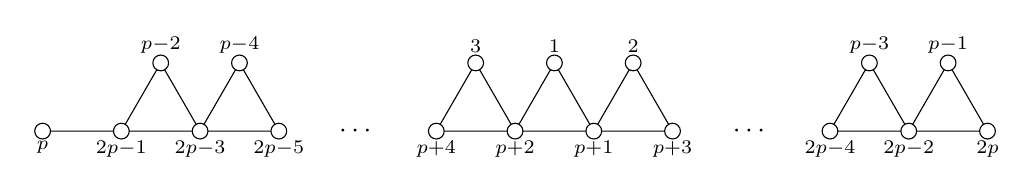
\begin{tikzpicture}
\draw(0,0)--(3,0)--(2.5,{sqrt(3)/2})--(2,0)--(1.5,{sqrt(3)/2})--(1,0);
\node[below]at(0,0){$\substack{p}$};\node[below]at(1,0){$\substack{2p-1}$};\node[below]at(2,0){$\substack{2p-3}$};\node[below]at(3,0){$\substack{2p-5}$};
\node[above]at(1.5,{sqrt(3)/2}){$\substack{p-2}$};\node[above]at(2.5,{sqrt(3)/2}){$\substack{p-4}$};
\node at(4,0){$\dotsb$};
\draw(5,0)--(8,0)--(7.5,{sqrt(3)/2)})--(7,0)--(6.5,{sqrt(3)/2})--(6,0)--(5.5,{sqrt(3)/2})--(5,0);
\node[below]at(5,0){$\substack{p+4}$};\node[below]at(6,0){$\substack{p+2}$};\node[below]at(7,0){$\substack{p+1}$};\node[below]at(8,0){$\substack{p+3}$};
\node[above]at(5.5,{sqrt(3)/2}){$\substack{3}$};\node[above]at(6.5,{sqrt(3)/2}){$\substack{1}$};\node[above]at(7.5,{sqrt(3)/2}){$\substack{2}$};
\node at(9,0){$\dotsb$};
\draw(10,0)--(12,0)--(11.5,{sqrt(3)/2)})--(11,0)--(10.5,{sqrt(3)/2)})--(10,0);
\node[below]at(10,0){$\substack{2p-4}$};\node[below]at(11,0){$\substack{2p-2}$};\node[below]at(12,0){$\substack{2p}$};
\node[above]at(10.5,{sqrt(3)/2}){$\substack{p-3}$};\node[above]at(11.5,{sqrt(3)/2}){$\substack{p-1}$};
\foreach\i in{0,1,2,3,5,6,7,8,10,11,12}{\draw[fill=white](\i,0)circle(0.1);}
\foreach\i in{1.5,2.5,5.5,6.5,7.5,10.5,11.5}{\draw[fill=white](\i,{sqrt(3)/2})circle(0.1);}
\end{tikzpicture}
\caption{Standard labeled triangular path $\tp_{2p}^I$   when $p$ is odd.}
\label{fig:tripathodd}
\end{figure}

\begin{figure}[H]
\centering
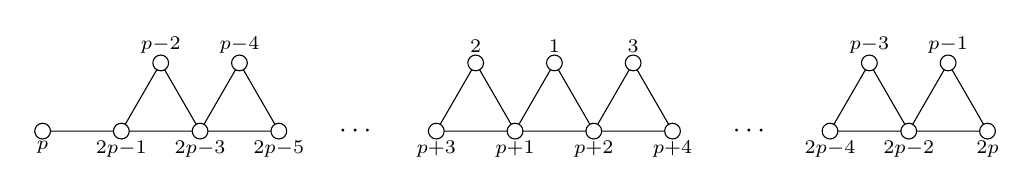
\begin{tikzpicture}
\draw(0,0)--(3,0)--(2.5,{sqrt(3)/2})--(2,0)--(1.5,{sqrt(3)/2})--(1,0);
\node[below]at(0,0){$\substack{p}$};\node[below]at(1,0){$\substack{2p-1}$};\node[below]at(2,0){$\substack{2p-3}$};\node[below]at(3,0){$\substack{2p-5}$};
\node[above]at(1.5,{sqrt(3)/2}){$\substack{p-2}$};\node[above]at(2.5,{sqrt(3)/2}){$\substack{p-4}$};
\node at(4,0){$\dotsb$};
\draw(5,0)--(8,0)--(7.5,{sqrt(3)/2)})--(7,0)--(6.5,{sqrt(3)/2})--(6,0)--(5.5,{sqrt(3)/2})--(5,0);
\node[below]at(5,0){$\substack{p+3}$};\node[below]at(6,0){$\substack{p+1}$};\node[below]at(7,0){$\substack{p+2}$};\node[below]at(8,0){$\substack{p+4}$};
\node[above]at(5.5,{sqrt(3)/2}){$\substack{2}$};\node[above]at(6.5,{sqrt(3)/2}){$\substack1$};\node[above]at(7.5,{sqrt(3)/2}){$\substack{3}$};
\node at(9,0){$\dotsb$};
\draw(10,0)--(12,0)--(11.5,{sqrt(3)/2)})--(11,0)--(10.5,{sqrt(3)/2)})--(10,0);
\node[below]at(10,0){$\substack{2p-4}$};\node[below]at(11,0){$\substack{2p-2}$};\node[below]at(12,0){$\substack{2p}$};
\node[above]at(10.5,{sqrt(3)/2}){$\substack{p-3}$};\node[above]at(11.5,{sqrt(3)/2}){$\substack{p-1}$};
\foreach\i in{0,1,2,3,5,6,7,8,10,11,12}{\draw[fill=white](\i,0)circle(0.1);}
\foreach\i in{1.5,2.5,5.5,6.5,7.5,10.5,11.5}{\draw[fill=white](\i,{sqrt(3)/2})circle(0.1);}
\end{tikzpicture}
\caption{Standard labeled triangular path $\tp_{2p}^I$  when $p$ is even.}
\label{fig:tripatheven}
\end{figure}

\begin{cor}
\label{tp_is_sympd}
For each integer $p\geq 2$, there exists a sympPD matrix in $ \symp(\tp_n^I)$.
\end{cor}

\bpf
Let $S=\begin{bmatrix}
    I & B_p\\
    O &I 
\end{bmatrix}$.
Then $N=S\trans S$ is a sympPD matrix.
It 
suffices to show that $\GL L(N)=\tp_{2p}^I$.

Observe that $N=\mtx{I & B_p\\B_p & I+B_p{^2} 
}$.  
Since $I$ is the leading $p\times p$ 
principal submatrix of $N$,
the set $\{1,\dots,p\}$ is an independent
set of vertices in $\G^L(N)$.  Edges in $\G^L(N)$  between $\{1,\dots,p\}$ and $\{p+1,\dots,2p\}$ are described by the nonzero entries of $B_p$. That is, the neighborhoods of vertices $1, \ldots, p$ are:  $N(1)=\{p+1,p+2\}$, $N(p)=\{2p-1\}$ and $N(i)=\{p+i-1,p+i+1\}$ for $i=2,\dots,p-1$.
Edges between vertices in $\{ p+1, \ldots, 2p\}$ are determined by the
dot products between columns of $B$. 
Thus, the edges in $G^L$ joining
pairs of vertices in $\{p+1, \ldots, 2p\}$ are $\{p+i, p+i+2\}$ for $i=1,\ldots, p-2$  and $\{p+1,p+2\}$. Hence $ \G^L(N)=\tp_{2p}^I$.
\epf




\subsection{Sparsity of inverse pairs of irreducible symmetric positive definite matrices}\label{ss:PDirred-sparse}

 The number of nonzero entries in a matrix $A$
is denoted by $\#(A)$.
 In this section we establish a lower bound on $\#(M)+\#(M^{-1})$ for an irreducible positive definite matrix $M$.  
Proposition \ref{sympd} then allows us to translate this to a lower bound for $\#(N)$ when $N$ is both symplectic and  positive definite, and triangular paths show this bound is sharp (see Corollary \ref{c:sympPD-sparseLB}). 

A symmetric  matrix $A$    is irreducible if and only if $\G(A)$ is connected.
 In the proof of the next theorem we use unlabeled graphs, although the graph of a matrix is technically a labeled graph; we suppress the labels since the labeling is irrelevant when discussing irreducible matrices because the class of irreducible matrices is invariant under permutations. 

 Note that if $M$ is an  irreducible symmetric invertible matrix, then $M^{-1}$ is also irreducible, so the graphs of $M$ and the graph of $M^{-1}$ are connected.
  



\begin{thm}\label{t:PDirred-sparseLB}
Let $M$ be an $n\times n$ irreducible, 
positive definite matrix. 
Then 
\[\#(M)+ \#(M^{-1}) \geq 8n-8.\]
\end{thm}

\begin{proof}
The proof is by induction on $n$.
{For $n=1$, $\#(M)+ \#(M^{-1})= 1+1 > 0=8\cdot 1 -8$.} 
For $n=2$, the irreducibility of $M$ implies 
that $\#(M) + \#(M^{-1})=4 +4 =8\cdot 2 -8$.

Now assume that $n>2$ and proceed by induction.
Throughout {this proof} we use $N$ to denote $M^{-1}$.  Since $M$ is positive definite, every diagonal entry is nonzero, so the number of nonzero vertices in row $i$ of $M$ is $1+\deg_{\G(M)}(i)$, and similarly for $N$.
If each vertex of $\G(M)$ and $\G(N)$ has degree at least 3, then 
\[ 
\#(M)+ \#(N) \geq 4n+4n=8n> 8n-8,
\]
as desired. Thus, we may assume that $\G(M)$ or $\G(N)$ 
has a vertex of degree at most $2$. We consider several cases. 

\bigskip\noindent
{\bf Case 1.} $\G(M)$ or $\G(N)$
has a vertex of degree $1$.

Without loss of generality, we can assume that  vertex
$1$ is a pendant vertex adjacent to  vertex $2$ in $\G(M)$.
Thus $M$ has the form 
\[
\begin{bmatrix}
m_{11} & m_{12} & 0 &\cdots & 0\\
m_{12} & m_{22} \\
0\\
\vdots\\
0 
\end{bmatrix}.
\]
 By considering the first row of the product  $MN=I$, we see that {$N_{\G(N)}[1]=N_{\G(N)}[2]$}. Since $\G(M)$, and hence $\G(N)$,
is connected and $n\geq 3$, vertex $1$ of $\G(N)$ has degree at least $2$. 

Let 
\begin{align*}
P&= \begin{bmatrix}
    1 & -m_{12}/m_{11}\\
    0 & 1
\end{bmatrix} \oplus I_{n-2},\\
\widehat{M}&= P\trans MP, \mbox{ and }\\
\widehat{N}&= P^{-1} N (P^{-1})\trans .
\end{align*}
Then 
$\widehat{M}$ and $\widehat{N}$ are
 positive definite matrices that are inverses of each other.  Examination of $\widehat{M}=P\trans MP$ shows that the  matrix $\widehat{M}$ has the form 
$[m_{11}] \oplus B$  where {(with the rows and columns of $B$ indexed by $2,\dots,n$)  $b_{22}=m_{22}-\frac{m_{12}^2}{m_{11}}$} and $b_{ij}=(M(1))_{ij}$ for $i,j\ge 2$ and $(i,j)\ne (2,2)$. Hence $\#(B)= \#(M(1))$.  Examination of $\widehat{N}=P^{-1} N (P^{-1})\trans$ shows that $\widehat{N}=
[1/m_{11}] \oplus N(1)$. 

Since $\G(M)$ is connected and vertex $1$ is a pendant vertex, $\G(M(1))$ is connected.
Hence $B$ is irreducible symmetric positive definite of order $(n-1)$ with inverse $N(1)$.
By induction, $\#(B) + \#(N(1))\geq 8(n-1)-8=8n-16$, implying that $\#(M(1))+ \#(N(1)) \geq 8n-16$.
The number of nonzeros in the first row and column of $M$ is 3, the number of nonzeros in the first row and column of $N$ is at least 5.
Therefore $\#(M)+ \#(N)\geq 8n-16 + 3 +5= 8n-8$,
as desired.


\bigskip\noindent 
{\bf Case 2.} All vertices of $\G(M)$ and $\G(N)$ have degree at least 2 and at least one has degree 2. 

Without loss of generality, we may assume that the neighbors of vertex $1$
in $\G(M)$ are vertices $2$ and $3$.  Thus $M$ has the form 
\[
M= \begin{bmatrix}
    m_{11} & m_{12} & m_{13} & 0 & \cdots & 0 \\
    m_{12}\\
    m_{13}
    \\
    0 \\
    \vdots\\
    0
\end{bmatrix}.
\]
Let 
\begin{align*}
P&= \begin{bmatrix}
    1 & -m_{12}/m_{11} & -m_{13}/m_{11}\\
    0 & 1 & 0 \\
    0 & 0 & 1
\end{bmatrix} \oplus I_{n-3},\\
\widehat{M}&= P\trans M P, \mbox{ and }\\
\widehat{N}&= P^{-1} N(P^{-1})\trans.
\end{align*}
Then $\widehat{M}$ and $\widehat{N}$ are symmetric positive definite matrices that are inverses of each other. Examination of $\widehat{M}=P\trans MP$ shows that  $\widehat{M}= [m_{11}] \oplus B$  where $b_{22}=-\frac{m_{12}^2}{m_{11}} + m_{22}$, $b_{23}=-\frac{m_{12}m_{13}}{m_{11}} + m_{23}$, $b_{33}=-\frac{m_{13}^2}{m_{11}} + m_{33}$, and $b_{ij}=m_{ij}$ for all other entries of $B$.
 Thus $\G(B)$ is  $\G(M(1))$ or is obtained from $\G(M(1))$ 
by deleting  or inserting  the edge joining vertices $2$ and $3$. Examination of $\widehat{N}=P^{-1} N (P^{-1})\trans$ shows that $\widehat{N}=
[1/m_{11}] \oplus N(1)$.  Since $B$ and $N(1)$ are inverses of each other, either   $\G(B)$ and $\G(N(1))$ are both connected or $\G(B)$ and $\G(N(1))$ are both disconnected.   

\bigskip\noindent
{\bf Subcase:} $\G(N(1))$ is connected.
\\
In this case, both  $\G(B)$  and $\G(N(1))$ are connected. So $B$ and $N(1)$ 
are irreducible, positive definite symmetric matrices of order $n-1$ 
and are inverses of each other. By induction, 
\[ \#(B) + \#(N(1))\geq 8(n-1)-8=8n-16.\]
The first row and column of $N$ contain at least $5$ nonzeros since all vertices of $\G(N)$ have degree at least $2$.
So $\#(N)\geq \#(N(1))+5$.  The first row and column of $M$ contain 
at least $5$ nonzeros, and $\#(M(1))\geq \#(B)-2$.  So, 
$\#(M) \geq \#(B)+3$.  It now follows that 
\[ \#(M) +\#(N) \geq 8n-16 + 5 + 3=8n-8,\] as desired. 

\bigskip\noindent
{\bf Subcase:} $\G(N(1))$ is disconnected.
\\
Since $B$ and $N(1)$ are inverses of each other, $B$ is also disconnected.  
Since $\G(B)$ and $\G(M(1))$ have the same edges except for possibly the edge joining $2$ and $3$, $\mathcal{G}(N(1))$ has exactly two 
connected components, one containing $2$ and 
the other containing $3$. Denote the vertex sets of the two connected components of $N(1)$ by $ \alpha$ and $ \beta$ where $2 \in \alpha$
and $3 \in \beta$.
Then  $M$ has the form 
\[ 
M= 
\left[ \begin{array}{ccc|c|c}
m_{11} & m_{12} & m_{13} & \mathbf 0^{\top} & \mathbf{0}^{\top}\\
m_{12} & m_{22} & m_{23} & \mathbf g^{\top} & \mathbf h^{\top} \\
m_{13} & m_{23} & m_{33} & \mathbf i^{\top} & \mathbf j^{\top}  \\ \hline
\mathbf 0 & \mathbf g &\mathbf i &  M[\alpha\setminus\{2\} ] & O 
\\ \hline 
\mathbf 0 & \mathbf h & \mathbf j &  O & M[\beta\setminus \{3\}] 
\end{array} \right] .  
\] 
and $N$ has the form 
\[
N= 
\left[ 
\begin{array}{ccc|c|c} 
n_{11} & n_{12} & n_{13} & \mathbf u^{\top} & \mathbf v^{\top} \\
n_{12} & n_{22}  & 0 & \mathbf x^{\top} & \mathbf 0^{\top}\\
n_{13} & 0 & n_{33} &  \mathbf 0^{\top} & \mathbf y^{\top} \\ \hline 
\mathbf u & \mathbf x &  \mathbf 0 &  N[\alpha\setminus\{2\}] & O \\ \hline 
\mathbf v & \mathbf {0} & {\mathbf y} & O & N[\beta
\setminus\{3\} ]
\end{array} 
\right] .
\] 
Note that  
\[ 
P^{\top}MP =
\left[ \begin{array}{ccc|c|c}
m_{11} & 0 & 0 & \mathbf 0^{\top} & \mathbf{0}^{\top}\\
0 & m_{22}-m_{12}^2/m_{11} & m_{23}-m_{12}m_{13}/m_{11} & \mathbf g^{\top} & \mathbf h^{\top} \\
0 & m_{23}-m_{12}m_{13}/m_{11} & m_{33}-m_{13}^2/m_{11}  & \mathbf i^{\top} & \mathbf j^{\top}  \\ \hline
\mathbf 0 & \mathbf g &\mathbf i &  M[\alpha\setminus \{2\} ] & O 
\\ \hline 
\mathbf 0 & \mathbf h & \mathbf j &  O & M[\beta\setminus \{ 3 \}] 
\end{array} \right] ,  
\] 
and 
$ P^{-1}N (P^{\top})^{-1} $
equals 
\begin{center}
\resizebox{.95\linewidth}{!}{$\left[ 
\begin{array}{ccc|c|c} 
 1/m_{11} & n_{12} + n_{22}m_{12}/m_{11} & n_{13} + n_{33}m_{13}/m_{11} & \mathbf u^{\top}+ (m_{12}/m_{11})\mathbf x^{\top}  & \mathbf v^{\top} + (m_{13}/m_{11}) \mathbf y^{\top} \\
n_{12}+n_{22}m_{12}/m_{11}  & n_{22} & 0 & \mathbf x^{\top} & \mathbf 0^{\top}\\
n_{13} +n_{33}m_{13}/m_{11} & 0 & n_{33} &  \mathbf 0^{\top} & \mathbf y^{\top} \\ \hline 
\mathbf u+ (m_{12}/m_{11})\mathbf x & \mathbf  x &  \mathbf 0 &  N[\alpha \setminus \{ 2\} ] & O \\ \hline 
\mathbf v + (m_{13}/m_{11})
\mathbf y & \mathbf {0} & \mathbf {y} & O & N[\beta\setminus \{3\} ]
\end{array} 
\right]$}.
\end{center}
Since $P^{\top} MP[\alpha , \beta]=O$, $m_{23}=m_{12}m_{13}/m_{11}$.  
Thus $m_{23} \neq 0$, that is,  there is an edge joining vertex $2$ and vertex $3$ in $\G(M)$. 
Since $P^{\top}MP$ and $P^{-1}N(P^{\top})^{-1}$ are inverses of each other, each off-diagonal entry in the first row of 
$P^{-1} N(P^{\top})^{-1}$\emph  is zero. 
Thus, 
\begin{align*}
n_{12}& =-n_{22}m_{12}/m_{11}\\
n_{13}&=-n_{33}m_{13}/m_{11}\\
\mathbf u& = -(m_{12}/m_{11}) \mathbf x \\ 
\mathbf v&= -(m_{13}/m_{11}) \mathbf y. 
\end{align*}
In particular, this implies for $j \in \alpha \setminus \{2\} $,  vertex  $j$ is a neighbor of vertex $2$ in $\G(N)$ if 
and only if $j$ is a neighbor of $1$ in $\G(N)$.
Since each vertex of $\G(N)$ has degree at least $2$, there is some $j \in \alpha \setminus \{2\} $ that  is a neighbor of vertex $2$. 
Hence vertex $1$ has at least two neighbors in $\alpha$. Similarly, vertex $1$ has at least two neighbors in $\beta$, and the degree $d$ 
of vertex $1$ in 
$\G(N)$ is at least $4$.


Up to permutation similarity, 
$B= B[\alpha]  \oplus B[\beta ]$
and $N(1)= N[\alpha] \oplus N[\beta]$. So $B[\alpha]$ and $B[\beta]$ are irreducible positive definite matrices of order $|\alpha|$ and $|\beta|$ respectively, and their inverses are $N[\alpha]$ and $N[\beta]$ respectively. 
Hence, by induction $\#(B[\alpha]) + \#(N[\alpha])\geq 8|\alpha| - 8$, and 
$\#(B[\beta]) + \#(N[\beta])\geq 8|\beta|-8$.


Note that $N$ has $1+ 2 {d}$ nonzero entries in its first row and column,  $M$ has $5$ nonzero entries in its first row and column, and $\G(B)$ is $\G(M(1))$ with exactly one edge removed.  
So $\#(M(1))=
\#(B)+2$. Hence, $\#(M) =\#(B[\alpha]) + \#(B[\beta])+7$.
It follows that 
\begin{align*} 
\#(M) +\#(N)  
&\geq \#(B[\alpha]) + \#(B[\beta]) +7 + \#(N[\alpha]) + \#(N[\beta]) + (1+ 2d)
\\
&= \#(B[\alpha]) + \#(N[\alpha])+ \#(B[\beta]) + \#(N[\beta]) +8 + 2d \\
&\geq 8|\alpha|-8+ 8|\beta|-8 + 8+ 2d \\
&=8(n-1) + 2d -8 
\\
&\geq 8n-8.
\end{align*}
\qedhere 
\end{proof}



\begin{cor}\label{c:sympPD-sparseLB} Let $n=2p$. 
Let $N$ be an  $n \times n$ sympPD matrix.  If $N$ is irreducible, i.e., $\G(N)$ is connected, then 
\[
\#(N) \geq 4n-4
\]
and $\G(N)$ has at least $3p-2$ edges. These bounds are sharp. 
\end{cor}

\begin{proof}
Assume $N$ irreducible.  Since $N$ is sympPD, $N^{-1}= \mtx{ N_{22}& -N_{12}\trans \\ 
-N_{12} & N_{11} }$ by Proposition \ref{sympd}.
Thus by Theorem \ref{t:PDirred-sparseLB},
$ 
2\#(N) = \#(N) + \#(N^{-1}) \geq 8(n-1),
$
and  the desired inequality follows. 

Since every diagonal entry of $N$ is positive and every edge is associated with two nonzero entries in the matrix, the number of edges in $\G(N)$ is $\frac 1 2(\#(N)-n)\ge 3p-2$ edges.
 Corollary \ref{tp_is_sympd} shows the bounds are sharp for $n\ge 4$.  A connected graph of order two has one edge, and $(3)(1)-2=1$.
\end{proof}



\subsection{Forbidden structures}\label{ss:forbid}

In this section  we seek conditions  that guarantee no matrix
with labeled graph $G^L$ is
sympPD.  First, we observe another property of sympPD matrices. 


\begin{prop}\label{cor:bigraphblock}
If 
\[ 
\renewcommand{\arraystretch}{1.1}
N=\left[ \begin{array}{cc}
A & B \\  
B\trans & C
\end{array}
\right]
\]
is sympPD, then 
$B$ is similar to a symmetric matrix; 
and hence each eigenvalue of  $B$ is real
and its algebraic and  geometric multiplicity are equal.   
\end{prop}

\bpf
Assume $N$ is {a sympPD matrix}. 
By Proposition \ref{sympd},  $A$ is positive definite, and there is a symmetric matrix $W$ with $B=AW$.  Since $A$ is positive definite, $A$ has a positive definite square root $\sqrt{A}$.  Note that 
$\sqrt{A}^{-1}B\sqrt{A}= \sqrt{A}W\sqrt{A}$, 
so $B$ is similar to the symmetric matrix $\sqrt{A}W\sqrt{A}$. The remainder of the proof follows from properties of similarity and real symmetric matrices. 
\epf


\begin{rem}\label{rem:NOallequal}
Proposition \ref{cor:bigraphblock} can be applied to exhibit examples of labeled graphs that do not allow all symplectic eigenvalues to be equal, or equivalently do not allow a sympPD matrix.
\begin{enumerate}
\item \label{NOallequal1}
If  a strongly connected component of the digraph $\Gamma^L(B)$ is a directed cycle  of length $\ell \geq 3$,
then each matrix with pattern $B$ has 
at least two non-real eigenvalues.  Hence, no $N$ of 
the form in Proposition \ref{cor:bigraphblock}
has all symplectic eigenvalues equal.
\item \label{NOallequal2}
If  $B$ has two irreducible components 
each equal to $[0]$ and there is a directed walk in $\Gamma^L(B)$ from one to the other, then every matrix with pattern $B$ has 0 as an eigenvalue with different algebraic and geometric multiplicities.  Hence no   $N$ of 
the form in Proposition \ref{cor:bigraphblock} with this $B$  has all symplectic eigenvalues equal. 
\end{enumerate}
\end{rem}




These examples suggest considering the maximum number of entries in a labeled graph that does not allow all eigenvalues to be equal.  The next example exhibits such a labeled graph of order $n=2p$ 
that omits $2p-1$ edges, i.e., that has $\binom{n}{2}-(n-1)=(p-1)(2p-1)$ edges.


\begin{ex}
\rm 
    Let $n=2p$ and let $G^L$ be the labeled graph with vertices $\{1,\dots,2p\}$ and edge set that is the complement of $\OL E=\{\{i,p+1\}\colon i=1,\dots,p\}\,\cup\,
    {\{\{i,p+2\}\colon i=2,\dots,p\}}$.  Let $N$ be a positive definite matrix whose labeled graph is $G^L$ and let $B=N[\{1,\dots,p\}, \{p+1,\dots,2p\}]$.  Then $B$ has two irreducible components 
each equal to $[0]$  and in the digraph there is an arc from one to the other.  Thus by Remark \ref{rem:NOallequal}\eqref{NOallequal2}, $N$ does not allow all symplectic eigenvalues to be equal.
\end{ex}

\begin{prop}\label{iso-isol}
    Let $G^L$ be a labeled graph that has an isolated vertex labeled $i$ and let $N\in\symp(G^L)$.  If the vertex labeled $i\pm p$ is not isolated, then $N$ has at least two distinct symplectic eigenvalues. 
\end{prop}
\bpf Without loss of generality assume $i=1$. We assume  $N=[n_{ij}]$ is a sympPD matrix and prove that  the vertex labeled $p+1$ is isolated.
  Recall that $(\Omega N)^2=-I$. The $(p+1)$-st row of $\Omega N$ is $(n_{11},0,\dots,0)$, so the $(p+1)$-st  row of $(\Omega N)^2$ is $-n_{11}$ times the first row of $\Omega N$. Thus $((\Omega N)^2)_{p+1,j}=-n_{1,1} n_{p+1,j}$. Since $((\Omega N)^2)_{p+1,j}=0$ for $j\ne p+1$, this implies $n_{p+1,j}=0$ for $j\ne p+1$, i.e., the vertex labeled $p+1$ is isolated.  
\epf


 There are also sparse 
labeled graphs that do not allow a sympPD matrix, e.g., a single edge and isolated vertices using a labeling where an isolated vertex is labeled 1 and an endpoint of the $K_2$ is labeled $p+1$.  Any tree is connected and if its order is at least four, then it has too few edges  {to allow a sympPD matrix} by Corollary \ref{c:sympPD-sparseLB}.

%%%%%%%%%%%%%%%%%%%%%%%%%%%%%%%%%%%%%%%%%%

\section{The Strong Symplectic Spectral Property (SSSP) and applications. }\label{s:strong} 


Like the inverse eigenvalue problem for graphs, the {symplectic inverse}  eigenvalue problem for labeled graphs may not behave well with respect to insertion of edges.  Namely,
 if  $A$ 
is a positive definite matrix and $H^L$ is a labeled graph obtained from the labeled graph  of $A$ by inserting some edges, then there may 
not be a matrix $B$ with labeled graph $H^L$ having the same 
symplectic spectrum as $A$.   In the IEP-$G$ setting, an additional constraint on $A$, known as the Strong Spectral Property, guarantees that if $H$ is a graph obtained from the graph of $A$ by inserting some edges,
then there is a matrix $B$ with graph $H$  
and the same spectrum as $A$.  In this section we establish a similar property in the symplectic setting  (Theorem \ref{supergraph}, the Supergraph Theorem), establish other extensions of IEP-$G$ results that use the Strong Spectral Property, develop the analogous theory, {and apply these ideas} to give several results about the  ISEP-$G$, including that every labeled graph $G^L$ of order $2p$ allows every set of $p$ distinct positive numbers as a symplectic spectrum. 
 

Throughout this section, we view the real $n\times n$ matrices as an inner product space, where the 
inner product between such matrices $A$ and $B$ is given by $\mbox{tr}(A^\top B)$. Note the set of symmetric $n\x n$ matrices, denoted by $\symm(n)$,
is a subspace, and for symmetric $A$ and $B$ the inner product simplifies to $\mbox{tr}(AB)$. 
 We will be working with subspaces of $\symm(n)$. For such a $U$ the {\it (symmetric) orthogonal complement}
of $U$ refers to 
\[ U^{\perp}=\{ A\in \symm(n)\colon\mbox{tr}(AB)= 0 
\mbox{ for all $B \in U$} \}; \]   
that is, the orthogonal complement with respect to $\symm(n)$. 


A reader who is familiar with the Strong Spectral Property of the IEP-$G$ and wishes to access the tools without first reviewing the theoretical foundation may wish to first read Definition \ref{d:SSSP} and the statement of Theorem \ref{SSSPequiv} and then proceed to Section \ref{ss:SSSPthms}.


\subsection{SSSP foundations}
The  $2p \times 2p$ matrices of the form 
\beq\label{Eq:HamForm}
M= \begin{bmatrix}
\begin{array}{cc}
R & E \\ 
F & -R^\top
\end{array} 
\end{bmatrix},
\eeq
where $R$ is a $p\times p$ real matrix, and  $E$ and $F$ are $p\times p$ real symmetric matrices
are called \textit{Hamiltonian matrices}. The set of $2p \times 2p$ Hamiltonian 
matrices {forms} a vector space, and is closed under the commutator $[\cdot, \cdot]$ (i.e., if $M$ and $M'$ are 
Hamiltonian matrices, then $[M,M']=MM'-M'M$ is a Hamiltonian matrix). 
Thus, the set of $2p\times 2p$ Hamiltonian matrices forms a Lie Algebra  with the commutator  as the bracket operator, and is denoted by $\spLA(2p)$. 
Additionally, it is known that if $M$ is a Hamiltonian matrix, then the exponential $e^M$ of $M$ is a symplectic matrix. 
Thus, the corresponding Lie group is $\Sp(2 p$), the group of $2p\times 2p$ symplectic matrices. 


\begin{defn}\label{d:SSSP}
The $2p\times 2p$ positive semidefinite matrix $N$  has the {\it Strong Symplectic Spectral Property} (SSSP) provided
\begin{equation}
\label{SSSP}
\{ NM+ M\trans N\colon M \in \spLA(2p) \} + \Span \mathcal{S}(\mathcal{G}^L(N))   = \symm(2p).
\end{equation}


In Theorem \ref{SSSPequiv} it is shown that  $N$ having the SSSP 
is equivalent to $Y=O$ {being} the only symmetric $2p\times 2p$ 
matrix for which $N\circ Y=O$ and {$\Omega NY=YN \Omega$}.
We note that the {IEP-$G$} analog of the SSSP is the Strong Spectral Property for 
a  symmetric matrix $A$ with graph $G$:
$
\{ AK+KA\colon K \in \Rnn\mbox{ and } K\trans=-K \} + \Span \SG= \symm(n).
$
This condition is equivalent to $Y=O$ being  
the only symmetric matrix 
such that $I \circ Y=O$, $A \circ Y=O$, and  $AY=YA$.
\end{defn}
\begin{ex}
Let $N=I_2$.
Then the labeled graph of $N$ is the empty graph on two vertices, and the subspace
\begin{equation}
\label{tangentspace} 
\{ NM + M\trans N\colon
M \in \spLA(2)\} 
\end{equation} 
 is the set of all $2\times 2$ symmetric matrices with trace equal to $0$. Furthermore  
$\Span \mathcal{S}(\mathcal{G}^L(N))$ is the set of all $2\times 2$ diagonal matrices. 
Thus $I_2$ has the SSSP. 
\end{ex}

\begin{ex}
Let $N=I_4$.  Then  for each $2\x 2$ matrix $R$ and 
all $2\x 2$ symmetric matrices $E$ and $F$, 
\begin{equation}
\label{eq:strongex}
N \left[ \begin{array}{cc}
R & E \\ 
F & -R\trans 
\end{array} \right]
+ \left[ \begin{array}{cc}
R & E \\ 
F & -R\trans 
\end{array} \right]\trans N=
\left[ \begin{array}{cc} 
R+ R\trans & E+F \\ 
E + F & -R-R\trans 
\end{array} 
\right]. 
\end{equation} 
Thus,  for each matrix in
\[ 
\{ NM + M^\top N\colon M \in \spLA(2p)\} 
+ \Span  \mathcal{S}(\mathcal{G}^L(N)),
\]
the $(1,2)$- and $(3,4)$-entries
are negatives of each other.  We conclude that $I_4$ does not have the SSSP. 
\end{ex} 


\begin{rem}
\label{rem:Gcomp}
Let $G^L$ be a labeled graph on $2p$ vertices and $N$ be a positive definite matrix 
with labeled graph $G^L$. The span $S$ of  $\sym(G^L)$ is the subspace of 
$\symm(2p)$ consisting of all $2p\times 2p$ matrices whose labeled graph
is a subgraph of $G^L$.  Thus, $S$ is spanned by the matrices  $E_{ij} + E_{ji}$ where $ij$ is an edge of $G^L$
and the matrices $E_{ii}$ $i=1, \ldots, 2p$. 
 It follows that the $2p\times 2p$ symmetric matrix $Y$ is in $S^{\perp}$ if and only if 
$Y_{ij}=0$ whenever $i=j$ or $ij$ is an edge of $G$. Since $ N\in\symp(G^L)$, it follows 
that $Y \in S^{\perp}$ if and only if $N\circ Y=O$. 
\end{rem}


\begin{lem}\label{lem:orthocomp}
Let $N$ be a $2p \times 2p$ positive definite matrix. 
The (symmetric) orthogonal complement of 
$ \{ NM+ M\trans N\colon M \in \spLA(2p) \}$  
is 
    \[\{Y\in\symm(2p)\colon \Omega NY=YN\Omega\}.\]
\end{lem}

\bpf 
From the definition, the (symmetric) orthogonal complement of  the first summand in
\eqref{SSSP} is 
\[ 
\{ Y \in \symm(2p)\colon
\tr(Y(NM+M\trans N))=0 
\mbox{ for all $M \in \mathfrak{sp}(2p)$} \}.
\]
Note that 
\begin{eqnarray*}
\tr(Y(NM + M\trans N)) &= & \mbox{tr}(YNM + YM\trans N) \\
& = & \tr(YNM + NMY)\\
& = & 2\tr(YNM).  
\end{eqnarray*}
The second inequality follows from the facts that { $\tr(A+B)=\tr(A)+\tr(B)$,} the trace of a matrix {equals the trace of} its transpose, and  both  $N$ and $Y$ are symmetric. 
The third inequality follows from the fact that 
$\mbox{tr}(AB)= \mbox{tr}(BA)$ for any appropriately sized matrices. 
Hence the {(symmetric)} orthogonal complement of 
the first summand in \eqref{SSSP}
is the set of symmetric matrices $Y$ such 
$YN \in \mathcal{W}$ {where $\mathcal{W}$ is the set of $2p\times 2p$
matrices such that $\tr(WM)=0$ for all $M \in \spLA (2p)$}.  


We  determine  the form of
\[
W= \begin{bmatrix}
    W_{11} & W_{12} \\
    W_{21} & W_{22}
\end{bmatrix}\in \mathcal{W},
\] where each $W_{ij}$ is $p\times p$.
Using the block form for a Hamiltonian matrix $M$ in \eqref{Eq:HamForm}, we see that $W\in \mathcal{W}$ if and only if 
$
\mbox{tr} (W_{11}R  + W_{12}F + 
W_{21}E-W_{22}R^\top)=0 $ for all symmetric  $E$ and $F$, and all $R\in\R^{p\x p}$. As $R$, $E$ and $F$ have no common positions, 
 $W \in \mathcal{W}$ if and only 
if $\mbox{tr}(W_{12}F)=0$ for all symmetric $F$, 
$\mbox{tr}(W_{21}E)=0$ for all symmetric $E$ and 
$\mbox{tr}((W_{11} - W_{22}^\top)R)=0$ for all $R$.
Thus, $W \in \mathcal{W}$ if and only if $W_{12}$ 
and $W_{21}$ are skew-symmetric, and  $W_{11}=W_{22}^\top$. 
One can verify that these  last conditions are equivalent to 
$ \Omega W^\top= W\Omega$. Therefore $\mathcal{W}$, which is the (symmetric) orthogonal complement of $ \{ NM+ M\trans N\colon M \in \spLA(2p) \}$,  is the set of symmetric matrices $Y$ such that
$\Omega N Y= YN \Omega$.
\epf



\begin{thm}
\label{SSSPequiv}
Let $N$ be a $2p\times 2p$ real positive definite matrix.
Then  $N$ has the SSSP if and only if $Y=O$ is the only symmetric matrix such that $N \circ Y=O$ and $ \Omega NY=YN\Omega$.
\end{thm}
\begin{proof}
The matrix $N$ has the  SSSP if and only if 
the orthogonal complements of the  two spaces in (\ref{SSSP}) intersect only in the zero matrix.  The theorem now follows from Remark \ref{rem:Gcomp} and Lemma \ref{lem:orthocomp}.
\end{proof}  


 We see that  the Strong Symplectic Spectral Property  for the complete graph  is similar to  the Strong Spectral Property for the complete graph: By the previous theorem, if $N\in\symp(K_{2p})$ then $N$ has the SSSP (for any labeling $L$ of $K_{2p}$), because $N\circ Y=O$ implies $Y=O$, just as in the case of the Strong Spectral Property  (and for the same reason{, since}   the condition $N\circ Y=O$ for any positive definite matrix $N$ implies $Y\circ I=O$). 


There are other labeled graphs for which every matrix has the SSSP, as seen in the next example.

\begin{ex}\label{ex:pK1veeKp-SSSP}
   Let  
$N\in\symp((\overline{K_{p}} \vee K_{p})^M)$ (cf. Example \ref{pK1veeKp}).  Then $N=\mtx{E & B\\B\trans & C}$ where $E$ is diagonal and every entry of $B$ and $C$ is nonzero, so $N\circ Y=O$ implies $Y=\mtx{X& O\\O& O}$ where $X$ is a symmetric $p\x p$ matrix.  Then $\Omega NY=YN\Omega$ implies $-EX=O$ and thus $X=O$. 

In contrast to the ISEP-$G$ and SSSP, there are matrices $A\in\symm(\OL{K_p}\vee K_p)$ that do not have the Strong Spectral Property for the IEP-$G$ and we exhibit one here. Let $A=\mtx{O & B\\B\trans & C}$ where $B=\mtx{
\begin{array}{rrrr}
-1 & -1 & -1 & -1\\3 & 3&3&3\\ -3 & -3&-3&-3\\1 & 1 & 1 & 1\end{array}}$ and $C$ is any $4\x 4$ symmetric matrix with every entry nonzero so that
$A\in\symm(\OL{K_p}\vee K_p)$.
For $Y=\mtx{X & O\\O & O}$  with $X=\mtx{0 &1& 4 & 9\\1 & 0 &1& 4\\4 & 1 & 0 & 1\\9 & 4&1&0}$, we have $Y\circ A=I\circ Y=O$ and $AY-YA=\mtx{O & -XB\\B\trans X & O}=\mtx{O & O\\O &  O}$, so $A$ does not have the Strong Spectral Property.
\end{ex}

 The matrix $\mtx{ I & B_p \\
      B_p & I + B_p^2 }\in \symp(\tp_{2p}^I)$, which is a sympPD matrix, fails to have the SSSP when $p=3$ as seen in the next example.

      \begin{ex}
           Let
          \[N=\mtx{ I & B_3 \\
      B_3 & I + B_3^2 }=\lb\begin{array}{cccccc}
 1 & 0 & 0 & 1 & 1 & 0 \\
 0 & 1 & 0 & 1 & 0 & 1 \\
 0 & 0 & 1 & 0 & 1 & 0 \\
 1 & 1 & 0 & 3 & 1 & 1 \\
 1 & 0 & 1 & 1 & 3 & 0 \\
 0 & 1 & 0 & 1 & 0 & 2 \\
\end{array}\rb \mbox{ and }Y=\lb\begin{array}{rrrrrr}
 0 & 1 & 0 & 0 & 0 & -1 \\
 1 & 0 & 2 & 0 & -1 & 0 \\
 0 & 2 & 0 & 0 & 0 & -1 \\
 0 & 0 & 0 & 0 & 0 & 0 \\
 0 & -1 & 0 & 0 & 0 & 1 \\
 -1 & 0 & -1 & 0 & 1 & 0 
\end{array}\rb\!.\]
Observe that $Y$ is symmetric, $Y\circ N=O$, and   $\Omega N Y=Y N \Omega$, so $N$ does not have the SSSP.   \end{ex}




In the next result, we use the SSSP formulation in Theorem \ref{SSSPequiv} to  characterize the positive definite diagonal matrices that have the SSSP. 





\begin{lem}\label{Diag}
Let 
$N= D \oplus E$ be a  $2p \times 2p$ positive definite diagonal matrix 
where $D=\diag(d_1, \ldots, d_p)$ and $E= \diag(e_1, \ldots, e_p)$. Then  the symplectic eigenvalues of 
$N$ {are $\sqrt{d_ie_i}, i=1,\dots,p$}, and $N$ has the SSSP if and only if the 
diagonal entries of $DE$ are distinct. 
In particular, if $D$ has distinct diagonal entries, then $\spspec(D\oplus D)=\{d_1, \ldots, d_p\}$ and $D \oplus D$ has SSSP. 
\end{lem}

\bpf
Since  
$(\Omega N)^2 = (-ED) \oplus -(DE) = - ( DE \oplus DE)$,  the symplectic eigenvalues of 
$N$ are $\sqrt{d_1e_1}, \ldots, \sqrt{d_pe_p}$.



 Let 
$
Y= \left[ \begin{array}{c c} W & X \\  
X\trans & Z  \end{array} \right]
$
be a $2p\times 2p $ symmetric matrix such that 
$\Omega NY= YN \Omega$ and $N\circ Y=O$.  The latter implies the diagonals  of $W$ and $Z$ are  zero.
Then $\Omega NY= YN \Omega$ implies
\begin{align}
EX\trans & = -XE,  \label{oneL} \\
-DX & = X\trans D, \label{twoL}\\
EZ& = WD, \mbox{ and } \label{threeL} \\
DW& = ZE. 
\label{fourL} 
\end{align}


First observe that \eqref{oneL} requires that every diagonal entry of $X$ is zero. Pre-multiplying both sides of \eqref{oneL} by $D$ and substituting in 
\eqref{twoL} yields $DEX\trans= X\trans DE$. If the diagonal entries of $DE$ are distinct, 
we conclude that the off-diagonal entries of $X$  are zero, i.e., $X=O$.

Let $W=[w_{ij}]$ and $Z=[z_{ij}]$. Examining the $(k,\ell)$ and $(\ell, k)$ entries of { \eqref{fourL}} and using the symmetry of $W$ and $Z$ gives
$d_kw_{k\ell}= e_\ell z_{k\ell}$ and 
$d_\ell w_{k\ell}= e_k z_{k\ell}$
These equations imply $w_{k\ell}=z_{k\ell}=0$ or $d_k e_k=d_\ell e_\ell$. Thus $N$ has the SSSP if the entries of $DE$ are distinct.
 
 
 Suppose that $N$ has a multiple symplectic eigenvalue. 
Then, without loss of generality, $d_1e_1=d_2e_2=1$.
Let $Y= e_{2}(E_{1,2} + E_{2,1}) + d_{1}(E_{ p+2,p+1} +E_{ p+1,p+2})$.
Then it can be verified that $Y$ is symmetric, $N\circ Y=O$ and $\Omega NY= YN\Omega $. 
\epf



\subsection{Fundamental theorems and consequences of the SSSP}\label{ss:SSSPthms}
In this section, we develop fundamental theorems about the SSSP.
The results and proofs, are analogous to those for the Strong Spectral Property. 
We place the proofs in the appendix for completeness. 


The criteria given in Definition \ref{d:SSSP} for a 
positive definite matrix $N$
to have the SSSP  can be phrased 
in terms of a system of linear equations by viewing the
entries $y_{ij}$ with $i\leq j$ as distinct variables.
This leads to an effective purely linear algebraic way to determine whether $N$ has the SSSP.  
More precisely, for a positive integer  $p$, we denote by $E_{ij}$ the $2p\times 2p$
matrix with a  {one} in position $(i,j)$ and zeros elsewhere. One can verify that 
\[ \{ E_{i, j+p}+ E_{j,i+p}: 1\leq i\leq j \leq p\}\cup
\{  E_{i+p,j}+E_{j+p,i}: 1\leq i\leq j \leq p\}
\cup \{  E_{ij}-E_{j+p,i+p} : 1\leq i,j \leq p\} 
\]
is a basis for $\spLA(2p)$. Thus $\spLA (2p)$ has dimension $ 2\frac{p(p+1)}2 +p^2= 2p^2 + p $.
As we need an ordered basis, we order this first as the order of the three sets just defined.  Within each of the first two sets we order by the pair $(i,j)$ running through diagonal (in order), followed by each superdiagonal in order.  For the third, each superdiagonal is followed by the corresponding subdiagonal. This index order for a $4\x 4$ matrix (with $p=2$ is $(1,1), (2,2), (1 , 2)$ for each of the first two  sets and $(1,1), (2,2), (1,2), (2,1)$ for the third.  This ordered basis is called the \emph{standard ordered basis} (for verification). 

Given an $2p\times 2p$ symmetric matrix $M$ we denote by 
$\uvec(M)$  the $(2p^2+p) \times 1$ vector obtained from $M$ by stacking (in  order) 
the upper triangular parts of columns of $M$.
If $M=[m_{ij}]$ is $4 \times 4$,  
\[ \uvec(M)^\top=
\left[ \begin{array}{cccccccccc}
m_{11} & m_{12}& m_{22}& m_{13} & m_{23} & m_{33} &
m_{14}& m_{24} & m_{34} & m_{44} 
\end{array} \right].
\] 
Note that $\uvec$ defines a bijection 
between  $(2p)\x(2p)$ symmetric matrices and $\mathbb{R}^{2p^2+p}$.

The {\it full SSSP verification matrix} of the $2p\times 2p$ positive definite matrix  $N$ is the  $ (2p^2\times p) \times (2p^2+p)$ matrix, $\Phi(N)$, whose columns are 
the {$\uvec (M^\top N + N M)$ where $M$}  runs over the standard ordered basis vectors of $\spLA(2p)$ {in order}  and the \emph{SSSP verification matrix}, $\Xi(N)$, of $N$ is the submatrix of rows  {indexed} by  the edges of $\Gc$. 

\begin{ex}\label{ex:verify}
Let 
$N=[n_{ij}]$ be  a $4\times 4$ symmetric matrix. 
Then $\Phi(N)$ equals
\[
\scriptscriptstyle{
\left[\begin{array}{cccccccccc}
0 & 0 & 0 & 4 \, n_{13} & 0 & 2 \, n_{14} & 2 \, n_{11} & 0 & 0 & 2 \, n_{12} \\
0 & 0 & 0 & 2 \, n_{23} & 2 \, n_{14} & n_{13} + n_{24} & n_{12} & n_{12} & n_{11} & n_{22} \\
0 & 0 & 0 & 0 & 4 \, n_{24} & 2 \, n_{23} & 0 & 2 \, n_{22} & 2 \, n_{12} & 0 \\
2 \, n_{11} & 0 & n_{12} & 2 \, n_{33} & 0 & n_{34} & 0 & 0 & -n_{14} & n_{23} \\
2 \, n_{12} & 0 & n_{22} & 0 & 2 \, n_{34} & n_{33} & -n_{23} & n_{23} & n_{13} - n_{24} & 0 \\
4 \, n_{13} & 0 & 2 \, n_{23} & 0 & 0 & 0 & -2 \, n_{33} & 0 & -2 \, n_{34} & 0 \\
0 & 2 \, n_{12} & n_{11} & 2 \, n_{34} & 0 & n_{44} & n_{14} & -n_{14} & 0 & -n_{13} + n_{24} \\
0 & 2 \, n_{22} & n_{12} & 0 & 2 \, n_{44} & n_{34} & 0 & 0 & n_{14} & -n_{23} \\
2 \, n_{14} & 2 \, n_{23} & n_{13} + n_{24} & 0 & 0 & 0 & -n_{34} & -n_{34} & -n_{44} & -n_{33} \\
0 & 4 \, n_{24} & 2 \, n_{14} & 0 & 0 & 0 & 0 & -2 \, n_{44} & 0 & -2 \, n_{34}
\end{array}\right]}\displaystyle{.}
\]
Here the rows correspond to entries 
$(1,1)$, 
$(1,2)$, $(2,2)$, 
$(1,3)$, $(2,3)$, $(3,3)$,  $(1,4)$, $(2,4)$, $(3,4)$ and $(4,4)$.
The columns correspond to 
$2E_{13}$, $2E_{24}$, $E_{14}+E_{23}$, $2E_
{3,1}$, $2E_{4,2}$, $E_{3,2}+E_{4,1}$, $E_{11} - E_{33}$, $E_{22}-E_{44}$, $E_{12}- E_{4,3}$ and $E_{21}-E_{3,4}$.

    
\end{ex}

\begin{ex}\label{ex:verify-cycle}

 Let $G^L$ be a cycle on four vertices  with the vertices labeled in cycle order; 
denote this by $G^L=C_4^I$. If $N\in\symp(C_4^I)$, then $\OL{C_4^I}$ has edges $\{1,3\}$  and $\{2,4\}$, so $n_{13}=n_{23}=0$ and all other entries are nonzero. Furthermore, 
\beq\label{eq:P4SSSP}
\Xi(N)=
\left[\begin{array}{cccccccccc}
2 \, n_{11} & 0 & n_{12} & 2 \, n_{33} & 0 & n_{34} & 0 & 0 & -n_{14} & n_{23} \\
0 & 2 \, n_{22} & n_{12} & 0 & 2 \, n_{44} & n_{34} & 0 & 0 & n_{14} & -n_{23} 
\end{array}\right].
\eeq
Examination of the {first and second} columns of $\Xi(N)$ shows  that the rows of $\Xi(N)$ are independent.  Thus Theorem \ref{t:verification} below shows that every positive definite matrix matrix $N$ with $\G^L(N)=C_4^I$ has the SSSP.
\end{ex}
\begin{thm} [{SSSP Verification Matrix}]
\label{t:verification}
Let $N$ be a $2p\times 2p$ positive definite matrix with labeled graph $G^L$. 
Then the following are equivalent
\ben[$(a)$]
\item \label{a:verification} $N$ has the SSSP.
\item \label{b:verification} 
The column space of $\Xi(N)$ spans $\mathbb{R}^{2p^2+p -|E(G)|}$.
\item \label{c:verification} The rows of $\Xi(N)$ are linearly independent. 
\een
\end{thm} 

 The proof is presented in Appendix \ref{appendix}. 
 It is more common to determine an SSSP verification matrix for a specific $N$, as in the next example.

\begin{ex}\label{KppSympPD-SSSP} 
Let 
$N=
\begin{bmatrix}
    1 & 0 & -1/\sqrt{2} & 1/\sqrt{2} \\0 & 1 & 1/\sqrt{2} & 1\sqrt{2} \\-1/\sqrt{2} & 1/\sqrt{2} & 2 & 0 \\1/\sqrt{2} & 1/\sqrt{2} & 0 & 2
\end{bmatrix}$
be  a $4\times 4$ symmetric matrix (observe $N$ is sympPD by Example \ref{KppSympPD}). 
 Then, using the same indexing as in the previous example,  
\[ \Xi(N)=\left[\begin{array}{rrrrrrrrrr}
0 & 0 & 0 & \sqrt 2 & \sqrt 2 & 0 & 0 & 0 & 1 & { 1} 
\\
\sqrt 2 & \sqrt 2 & 0 & 0 & 0 & 0 & 0 & 0 & -2 & -2 
\end{array}\right].
\] 
Here the rows of $\Xi(N)$ correspond to 
entries $(1,2)$ and $(3,4)$ of $N$.
Note that $\Xi(N)$ has rank 2, and hence $N$ has the SSSP.   Observe that $\G^L(N)=K_{2,2}^M$. 
\end{ex}

The following shows that the set of positive definite $2p\times 2p$ matrices with the SSSP is an open subset of {$\symm(2p)$}. 
Here $\| M\|$ denotes any fixed 
induced matrix norm, e.g., the spectral norm.

\begin{cor}
\label{open}
Let $N$ be a $2p\times 2p$ positive definite matrix with the SSSP.
Then there exists $\epsilon>0$  such that every {symmetric} matrix   $M$ with 
 $\|N-M \|<\epsilon$ is positive definite and has the SSSP. 
\end{cor}

\begin{proof}
Note that  $\Phi(N)$ is a 
continuous function of the entries of $N$.
So for symmetric $M$ sufficiently close to $N$, 
$M$ is positive definite and $\G(M)$ is supergraph of $\G(N)$. Thus the rows of $\Xi(M)$ 
are a subset of the rows of $\Xi(N)$. 
Hence the rows of $\Xi(M)$ are linearly independent.  
By Theorem \ref{t:verification}, $M$ has the SSSP. 
\end{proof}

The next two results show that if a labeled graph allows a positive definite matrix 
with a given symplectic spectrum, then each labeled graph obtained by inserting edges allows a 
positive definite matrix with the same symplectic spectrum. 

\begin{thm}{\rm \bf (Supergraph Theorem)}
\label{supergraph}
\\
Let $N$ be a  $2p\times 2p$ positive definite matrix having the SSSP and   labeled graph $G^L$. 
Let $H^L$ a labeled graph on $2p$ vertices obtained from $G^L$ by inserting some edges.
Then there exists a matrix  with  
labeled graph $H^L$ having the same symplectic eigenvalues as $N$ and also having the SSSP.
\end{thm}

The proof of the Supergraph Theorem is similar to that used for the analogous IEP-$G$ result and can be found in Appendix \ref{appendix}.


\begin{cor}\label{AllSimple}
    Every labeled graph of order $n=2p$ allows 
    every set of $p$ distinct positive real numbers as the symplectic spectrum of matrix with the SSSP.
\end{cor}
\begin{proof}
Let $\lam_1, \ldots, \lam_p$ be distinct positive real numbers, and $D= \diag(\lam_1, \ldots, \lam_p)$.
Then by Lemma \ref{Diag}, $D \oplus D$ is a positive definite matrix with the SSSP whose labeled graph is 
the empty graph on $2p$ vertices.  The result now follows from Theorem \ref{supergraph}.
\end{proof}



The next theorem  is an analog of a main result for the Strong Spectral Property and the IEP-$G$.  Its proof is in Appendix \ref{appendix}.

\begin{thm}\label{Thm:bifurcation}{\rm \bf (Bifurcation Theorem) }
\\
Let $N$ be a $2p \times 2p$ positive definite matrix having the SSSP.  
Then there exists $\epsilon>0$ such that if $\widehat{N} $ is a $2p\times 2p $ positive definite matrix 
with $\| \widehat{N}- N \| <\epsilon$, then there exists a 
matrix  $N'\in \symp(\G^L(N))$ such that $\spspec(N')=\spspec(\wh N)$.
\end{thm}

\begin{cor}\label{c:bifur-close}
Let $N$ be a  positive definite matrix $2p\times 2p $ with the SSSP and $\spspec(N)=\{\lam_1,\dots,\lam_p\}$. 
Then there exists $\delta>0$   {with the property that}   for every list $\alpha=\{\hat\lam_1,\dots,\hat\lam_p\}$ of $p$ positive real numbers such that $|\hat\lam_i-\lam_i|<\delta$ for $i=1,\dots,p$,  there is a matrix $N'\in \symp(\G^L(N))$ such that $\spspec(N')=\alpha$.
\end{cor}
\bpf We use the spectral norm.
Let $S$ be a symplectic matrix such that $S\trans NS=D\oplus D$ where $D=\diag(\lam_1,\dots,\lam_p)$.
Use Theorem \ref{Thm:bifurcation} to choose $\epsilon>0$  such that if $\widehat{N} $ is a $2p\times 2p $ positive definite matrix 
with $\| \widehat{N}- N \| <\epsilon$, then there exists a matrix  $N'\in\symp(\G^L (N))$ such that
 $\spspec(N')=\spspec(\widehat{N})$. Define $\delta=\frac\epsilon{\|S^{-1}\|^2}$. Let $\alpha=\{\hat\lam_1,\dots,\hat\lam_p\}$ be such that $|\hat\lam_i-\lam_i|<\delta$ for $i=1,\dots,p$.  Define $\wh D=\diag(\hat \lam_1,\dots,\hat \lam_p)$ and $\wh N=((S^{-1})\trans(\wh D\oplus \wh D)S^{-1}$ and observe that $\spspec(\wh N)=\alpha$.  Then 
\begin{align}\nonumber
\|\wh N-N\|&=\|((S^{-1})\trans((\wh D-D)\oplus (\wh D-D)) S^{-1}\|\\ 
\nonumber
&\le \|(S^{-1})\trans \| \|(\wh D-D)\oplus (\wh D-D)\| \|S^{-1}\|< \| S^{-1}\|^2\delta=\epsilon.
\end{align} 
Thus by Theorem \ref{Thm:bifurcation}, there exists a positive definite  matrix $N'$  with $\G^L(N')=\G^L(N)$ and $\spspec(N')=\spspec(\widehat{N})=\alpha$. \epf

  Given a positive definite matrix $N$ we list its distinct symplectic eigenvalues in increasing order 
$\lambda_1<  \lambda_2< \cdots< \lambda_q$.
  The \textit{ordered symplectic multiplicity} list of $N$ 
is  $\soml(N)=(m_1, \ldots, m_q)$  where $m_i$ is the multiplicity of $\lambda_i$
as a symplectic eigenvalue of $N$.  A \emph{refinement} of $\soml(N)$ is a list obtained from $\soml$ by replacing
each $m_i$ with a partition of $m_i$. 
 The next result is immediate from Corollary \ref{c:bifur-close}.

 
\begin{cor}\label{cor:bifurcationSMP}{\bf (Bifurcation Corollary for Multiplicity Lists)}
\phantom{ } \\
    Let $N$ be a positive definite matrix with the SSSP.  Then for each refinement $\soml'$ of $ \soml(N)$, there is a positive definite matrix $N'$ with the SSSP, { $\G^L(N')=\G^L(N)$,}  and $\soml({N'}) = \oml'$. 
In particular,    if all the symplectic eigenvalues of $N$ are equal, then {$\G^L(N)$}  allows every possible ordered symplectic multiplicity list. 
\end{cor}



The next result can be used to  solve  certain ISEP-$G$ problems even when a given matrix 
does not have the SSSP. 
A few definitions are needed.
Let $N$ be a $2p \times 2p$ positive definite matrix
with labeled graph $G^L$.  Then $N$ defines a subspace
\begin{equation}
\label{eq:tanf}
\{ NM + M^\top N : M \in \spLA(2p) \}. 
\end{equation} 
Let $R=[r_{ij}]$ be a matrix in the subspace defined in \eqref{eq:tanf}.
The \textit{labeled graph of $G^L$ in the direction of $R$} 
is denoted by $G^L_R$ and is obtained from $G^L$ by inserting 
an edge joining $i$ and $j$, if not already present, whenever
$r_{ij} \neq 0$ and $i\neq j$.
We say that \textit{$N$ has the SSSP
with respect to $G^L_R$} provided 
\[ 
 \{NM+ M^\top N\colon M \in \spLA(2p) 
\} + \{ B \in \Span (\mathcal{S}(G^L_R))\}= \symm(n).
\]
This is equivalent to $Y=O$ is the only symmetric matrix such that $N \circ Y=O$, 
$R \circ Y=O$ and $\Omega NY=YN\Omega$.


\begin{thm}\label{liberation}{(\bf Matrix Liberation Lemma)}
\phantom{ } \\
Let $N$ be an $n\times n$ positive definite matrix with labeled graph $G^L$, $R$ be a matrix in {the subspace in} $(\ref{eq:tanf})$ 
and  $G^L_R$ be the labeled graph of {$G^L$} in the direction of $R$.
If $N$ has the SSSP with respect to $G^L_R$, then there is a positive 
definite matrix  with labeled graph  $G^L_R$ that has the same  symplectic eigenvalues as $N$ and has the SSSP. 
\end{thm}



\begin{ex}
Here we illustrate the use of the Matrix Liberation Lemma. 
Let 
\[ 
A=\begin{bmatrix}
\begin{array}{rrr}
2 & -1 & 0 \\
-1 & 2 & -1 \\
0 & -1 & 2
\end{array}
\end{bmatrix} ,  
 B= \begin{bmatrix} 
 \begin{array}{rrr}
2 & 1 & 0 \\
1 & 3 & 1 \\
0 & 1 & 2
\end{array}
\end{bmatrix}
\mbox{ and } 
N= A \oplus B. 
\] 
Then  $\det(xI-\Omega N)=x^2 I + AB$ and
\[
AB=
\begin{bmatrix}
 \begin{array}{rrr}
3 & -1 & -1 \\
0 & 4 & 0\\
-1 & -1 & 3
\end{array} 
\end{bmatrix}
\] 
 has eigenvalues  $2, 4,4$.
It follows that the symplectic eigenvalues of $N$  are  $\sqrt{2}$, $2$ and $2$.

{Observe that \[Y=
\begin{bmatrix}
\begin{array}{rrrrrr}0 & 0 & 0 & -1 & 2 & -1 \\
 0 & 0 & 0 & -2 & 0 & 2 \\
 0 & 0 & 0 & 1 & -2 & 1 \\
 -1 & -2 & 1 & 0 & 0 & 0 \\
 2 & 0 & -2 & 0 & 0 & 0 \\
 -1 & 2 & 1 & 0 & 0 & 0 \end{array} \end{bmatrix}\] shows that $N$ does not have the SSSP.}

Let 
\[ 
M=\frac{1}{3}
\begin{bmatrix}
\begin{array}{rrrrrr}
0 & 0 & 0 & 0 & {5} & {4} \\
0 & 0 & 0 & {5} & {5} & {2} \\
0 & 0 & 0 & {4} & {2} & 0 \\
{4} & -3 & 0 & 0 & 0 & 0 \\
-3 & 0 & 0 & 0 & 0 & 0 \\
0 & 0 & {1} & 0 & 0 & 0
\end{array}\end{bmatrix}.
\] 
Then $M\in \spLA(6)$, 
and 
\[
R:=M\trans N+NM =
\begin{bmatrix}
    0 & 0 & 0 & 0 & 0 & 1\\
    0 & 0 & 0 & 0 & 0 & 0 \\
    0 & 0 & 0 & 1 & 0 & 0\\
    0 & 0 & 1 & 0 & 0 & 0 \\
    0 & 0 & 0 & 0 & 0 &0 \\
    1 & 0 & 0 & 0 & 0 &0
\end{bmatrix}. 
\]
To show that $N$ has the SSSP with respect to $G^L_R$,
let   $Y$ be a matrix of the form 
\[ 
\begin{bmatrix} 
\begin{array}{rrrrrr}
0 & 0 & a & b & c & 0 \\
0 & 0 & 0 & d & e & f \\
a & 0 & 0 & 0 & g & h \\
b & d & 0 & 0 & 0 & i \\
c & e & g & 0 & 0 & 0 \\
0 & f & h & i & 0 & 0
\end{array}\end{bmatrix} 
\] 
with $\Omega NY=YN\Omega$. 
Then 

\begin{center}
\resizebox{\linewidth}{!}
{$
\begin{bmatrix}\begin{array}{cccccc}
4 \, b + 2 \, c & b + 3 \, c + 2 \, d + e & c + g & 0 & a & -2 \, a + 2 \, i \\
b + 3 \, c + 2 \, d + e & 2 \, d + 6 \, e + 2 \, f & e + 2 \, f + 3 \, g + h & i & 0 & i \\
c + g & e + 2 \, f + 3 \, g + h & 2 \, g + 4 \, h & -2 \, a + 2 \, i & a & 0 \\
0 & i & -2 \, a + 2 \, i & -4 \, b + 2 \, d & b - 2 \, c - 2 \, d + e & d + f \\
a & 0 & a & b - 2 \, c - 2 \, d + e & 2 \, c - 4 \, e + 2 \, g & e - 2 \, f - 2 \, g + h \\
-2 \, a + 2 \, i & i & 0 & d + f & e - 2 \, f - 2 \, g + h & 2 \, f - 4 \, h
\end{array}\end{bmatrix}
$}
\end{center}
equals $O$. It can be verified that this occurs if and only if $Y=O$.  Hence $N$ has the SSSP with respect to $G^L_R$. 
The Matrix Liberation Lemma now implies that there is a matrix having the SSSP 
whose labeled graph is that of $N$ in the direction of $R$ 
with the same symplectic spectrum as $N$.  
Hence the 6-cycle with  the cyclic order labeling 
allows a matrix having the SSSP with a multiple symplectic eigenvalue. 
\end{ex}


 %%%%%%%%%%%%%%%%%%%%%%%%%%%%%%%%%%%%%%%%%%


\section{Symplectic spectrally arbitrary labeled graphs}\label{s:ssa} 


A labeled graph $G^L$ of order $n=2p$  is \emph{symplectic spectrally arbitrary} if for any $p$ positive numbers $\lam_1,\dots,\lam_p$, there is a   matrix $N\in\symp(G^L)$ such that $\lam_1,\dots,\lam_p$ are the symplectic eigenvalues of $N$.




In this section, we use the construction $N=S\trans D'S$ where  $S$ is a  symplectic matrix  and  $D'=D\oplus D$ is a diagonal matrix
with a desired symplectic spectrum  to construct  a variety of labeled graphs that are symplectic spectrally arbitrary. In particular, we  show that the sparse labeled graph  $\tp_n^I$ is symplectic spectrally arbitrary 
for each positive even integer $n=2p$. 
Additionally, we show that a  variety of dense labeled graphs, including  $K_{n}$, 
are symplectic spectrally arbitrary. 



We begin with a result about nonnegative symplectic matrices that shows the existence of many symplectic spectrally arbitrary labeled graphs.


\begin{prop}\label{l:nonnegsymplectic}
 Let $S$ be a  nonnegative symplectic  matrix  and let $G^L=\GL L(S^\top S)$.
  Then $G^L$ is symplectic spectrally arbitrary.
\end{prop}

\begin{proof} Assume $S$ is $(2p)\x(2p)$, let $n=2p$, let $D$ be a $p\x p$ diagonal matrix with positive diagonal entries,  let $D'=D\oplus D$, and define $N=S^\top D'S$. Then  the  symplectic eigenvalues of $N=[n_{ij}]$ are the diagonal entries of $D$. Note that \[ 
n_{ij}=\sum_{r=1}^n s_{r i}d'_{rr}s_{r j}
\]
Since all entries of $S$ are nonnegative and all entries $d'_{rr}$ are positive, $n_{ij}\neq0$ if and only if there exists $1\leq r\leq n$ such that $s_{r i}s_{r j}\neq0$. This is equivalent to $(S^\top S)_{ij}=\sum_{r=1}^n s_{r i}s_{r j}\neq0$. Hence, $N\in \symp(G^L)$ and $G^L$ is symplectic spectrally arbitrary.
\end{proof}
 

\begin{rem}\label{manySSA}
Proposition \ref{l:nonnegsymplectic} together with the indicated prior result shows that   each of the following  labeled graphs is symplectic spectrally arbitrary for every positive integer $p$: $(\OL{K_p}\vee K_p)^{M}$ (Example \ref{pK1veeKp}) and 
    $(\tp_{2p})^I$ (Corollary \ref{tp_is_sympd}).  
\end{rem}


{We can generalize the method in Proposition \ref{p:IBOBsympPD}. 

\begin{prop}\label{IBOIisSSA} Let $B=[b_{ij}]$ be a symmetric $p\times p$ matrix,  $S=\mtx{I &  B\\O & I}$,   $N=S\trans S$ and  $G^L=\G^L(N)$.  Then $G^L$ is symplectic spectrally arbitrary.
\end{prop}
\bpf By Proposition \ref{p:IBOBsympPD}, $N=\mtx{I & B \\B & I+B^2}$. For {positive real numbers} $\lam_1,\dots,\lam_p$,  define $D=\diag(\lam_1,\dots,\lam_p)$ and $D'=D\oplus D$.  Use $B$ and $D$ to define 
    $\wt B=\sqrt D^{-1}B \sqrt D^{-1}$,   $\wt S=\mtx{I & \wt B\\O & I}$, and $\wt N=\wt S\trans D' \wt S$.  Then $\wt S$ is symplectic and  $\spspec({\wt N})=\{\lam_1,\dots,\lam_p\}$.  Furthermore,
\[ 
\wt N=\wt S\trans D' \wt S=\mtx{D & D\wt B \\
       \wt B D &  D+\wt B D\wt B }=
       \mtx{D & \sqrt D B \sqrt D^{-1}\\
       \sqrt D^{-1} B\sqrt D & D+\sqrt D^{-1}B^2 \sqrt D^{-1}}\in \symp(G^L). \qedhere
\] 
\epf
The next result is immediate from Proposition \ref{IBOIisSSA} and Example \ref{KppSympPD}.
\begin{cor}\label{KppSSA}
The labeled graph $K_{p,p}^M$ is  symplectic spectrally arbitrary.
 \end{cor}
}


The complete graph is also symplectic spectrally arbitrary, as seen in the next example.

\begin{ex}\label{random}
Given an arbitrary multi-set $\{\lam_1,\dots,\lam_p\}$ of positive real numbers, we create a positive definite matrix $N$ with this set of symplectic eigenvalues
whose labeled graph is either $ K_{2p}$ or 
$(K_{p}\du K_p)^I$ where the label $I$ indicates that the vertices
of the first $K_p$ are labeled by $1, \ldots, p$.
We accomplish this by using `random' symplectic matrices to `smear' the entries of $D'=\mtx{D  & O\\ O&D}$ where $D=\diag(\lam_1,\dots,\lam_p)$. 

Specifically, let $A$ be a random 
 $p\x p$ matrix.  With high probability $A$ is invertible,   $S_A=\mtx{A & O\\O & (A^\top )^{-1}}$ is a symplectic matrix and $S_A^\top D'S_A=\mtx{A^\top D A & O\\ O & (A^{-1})D (A^\top )^{-1}}$ is 
 a positive definite matrix with symplectic eigenvalues $\lambda_1, \ldots, \lambda_p$.
Since $A$ is chosen randomly (and for this set of symplectic eigenvalues),     $\GL L(S_A^\top D'S_A)\cong (K_p\du K_p)^I$ with high probability.  Thus the labeled graph  $(K_p\du K_p)^I$  is symplectic spectrally arbitrary. 

Next let $B$ be a random $p\x p$ symmetric matrix, i.e., the entries of $B$ on the diagonal and above are chosen randomly. Then  $R_B=\mtx{I & B\\O & I}$ is a symplectic matrix and $R_B^\top S_A^\top D'S_AR_B=\mtx{A^\top D A & A^\top D AB\\B A\trans D A & BA^\top D AB+(A^{-1})D (A^\top )^{-1}}$. 
Since $A$ and $B$ are chosen randomly, 
the labeled graph of $(R_AS_B)^\top D'S_AR_B$ is $K_{2p}$ with high probability. 
\end{ex} 


As noted in Section \ref{s:strong},  $N\in\symp(K_{2p})$ implies $N$ has the SSSP for any labeling $L$ of $K_{2p}$.  
However, not every matrix constructed by 
 the `random' method in {used} Example \ref{random} has the SSSP, as seen in the next  example.
 
\begin{ex}\label{random-notSSSP}
    A matrix $N\in\symp((K_p\du K_p)^I)$  constructed as in Example \ref{random} with all symplectic eigenvalues equal to one has the form $N=\mtx{A & O\\O & A^{-1}}$ where $A$ is positive definite (we have replaced $A\trans IA$ with $A$ arbitrary by $A$ with $A$ positive definite).  Applying Theorem \ref{SSSPequiv} we see that $Y\circ N=O$ implies $Y=\mtx{O & X\\X^T & O}$. Then $\Omega NY=Y N \Omega$ is  equivalent to $X\trans A=-AX$ (because this implies  $A^{-1}X\trans=-XA^{-1}$). This is equivalent to $X\trans A+AX=O$, which is a homogeneous system of  
    $\frac{p(p+1)}2$ linear equations in  $p^2$ variables, so {there exists} a nonzero solution $X$, 
    {and $N$ does not have the SSSP}. 
\end{ex}



We also observe that there are graphs that do not have any labeling that is symplectic spectrally arbitrary because they have too few edges.

\begin{rem}\label{notSSA}
     Any labeled graph that does not allow a sympPD matrix does not allow all eigenvalues equal, and so is not symplectic spectrally arbitrary. In particular, if $G$ is a graph of order $n=2p$ and $|E(G)|<3p-2$, then $G^L$ is not symplectic spectrally arbitrary for any labeling $L$ of $G$ by Corollary \ref{c:sympPD-sparseLB}.  This includes trees for $n\ge 4$ and unicyclic graphs for $n\ge 6$.
\end{rem}



      
As noted in Remark \ref{manySSA}, the graph $\tp^I$ is symplectic spectrally arbitrary, showing  that $3p-2$ is the minimum number of edges in a symplectic spectrally arbitrary graph $G^L$ of order $2p$.

%%%%%%%%%%%%%%%%%%%%%%%%%%%%%%%%%%%%%%%%%

\section{Symplectic  eigenvalues of order four graphs}\label{s:order4}
In this section we determine the possible symplectic eigenvalues  of each of the eleven graphs of order four.  To do this, we develop several additional tools for determining symplectic spectra, some of which are applications of strong properties. We begin with a remark that greatly simplifies this problem by applying the machinery we have developed. 


\begin{rem}\label{o4sympPD3SSA}
    For $n=4$ there are only two eigenvalues and thus only two possible multiplicity cases: two equal or two distinct symplectic eigenvalues.  Since every labeled graph allows all possible distinct symplectic spectra (by Corollary \ref{AllSimple}), solving the ISEP for a labeled graph $G^L$ of order four is equivalent to determining whether $G^L$ allows a sympPD matrix; if so, it is symplectic spectrally arbitrary. 

Thus  every labeling of    $K_4$ is symplectic spectrally arbitrary {(with the SSSP)} by Example \ref{random}, $ ({\OL{K_2}}\vee K_2)^{M}$ (with the SSSP) by Example \ref{ex:pK1veeKp-SSSP}, and $K_{2,2}^{M}$  (with SSSP) by Example \ref{KppSympPD-SSSP}. 
By Corollary \ref{c:sympPD-sparseLB}, any connected graph on four vertices with fewer than four  edges does not allow a sympPD and thus has all symplectic eigenvalues simple.  Therefore, each labeling of $P_4$ and $K_{1,3}$ allows any set of two distinct symplectic eigenvalues and no other symplectic spectra.
\end{rem}



Among connected graphs, this leaves  the Paw graph, shown in Figure \ref{fig:paw-couple}, for which the symplectic eigenvalues need to be determined for various labelings,  and  other labelings of   $K_4-e\cong 2K_1\vee K_2$ and $C_4\cong K_{2,2}$. 



So far we have been working entirely with labeled graphs. 
 However, many labelings must result in the same symplectic eigenvalues because they can be obtained from one another by symplectic permutation matrices or other symplectic matrices 
 that preserve the unlabeled graph; we call such labelings \emph{symplectically equivalent}.   When determining all symplectic eigenvalues of all graphs of a given order, it is desirable to consider only one representative from each class of symplectically equivalent labelings of a graph $G$.


A \textit{monomial matrix} is  a $(0,1,-1)$-matrix $R$ with exactly one nonzero in each row and column. 
Each monomial matrix has the form $R=EP$ where $E$ is a diagonal matrix each of whose diagonal entries are in $\{\pm 1\}$, 
and $P$ is a permutation matrix; note that $R\trans=R^{-1}$ for  each monomial matrix $R$. Let $R$ be a monomial matrix for which $R^{\top}{\Omega}R=\Omega$, and let $N$ be a positive definite matrix.
By Proposition \ref{sympev}, the  symplectic eigenvalues of $N$ 
are the moduli of the eigenvalues of $\Omega N$.
Note that $\Omega N= R^{\top} \Omega R N$ is similar to $\Omega R N R^{\top} $, so $N$ and $RNR^{\top}$ have the same symplectic eigenvalues. Therefore, if  $R=EP_\sigma$ and the labeled graph of $N$ is $G^L$, then $ \G^L(RNR^{\top})=\G^L(P_{\sigma} NP_{\sigma}^{\top})=G^{\sigma(L)}$. 
In other words, for such $\sigma$, 
studying the symplectic eigenvalues of matrices with labeled graph $G^{L}$ is  the same as studying the symplectic eigenvalues of matrices with labeled graph $G^{\sigma(L)}$. 

To identify  graphs  $G^{\sigma(L)}$ that allow the same symplectic spectra as $G^L$,  we need to find  the permutation matrices $P$ so that 
\[ 
\left[
\begin{array}{cc}
O & I\\
I & O  
\end{array}
\right]
\left[ \begin{array}{cc} 
 P_{11} &  P_{12} \\
 P_{21} & P_{22} 
 \end{array} \right] 
 = 
\left[ \begin{array}{cc} 
 P_{11} &  P_{12} \\
 P_{21} & P_{22} 
 \end{array} \right] 
 \left[
\begin{array}{cc}
O & I\\
I & O  
\end{array}
\right].
\] 
This is equivalent to $P_{21}=P_{12}$  and $P_{11}=P_{22}$. 
If the permutation corresponding to $P$ is $\sigma$, one can check that this implies 
$\sigma(i) = j$  if and only if $\sigma(i+p)=j+p$ (reading indices mod $2p$).  So the permutations $\sigma$ that work are those such that 
\[ \{ \{ \sigma(1), \sigma(1+p)\}, \ldots, \{ \sigma(p), \sigma(2p)\} \}= \{ \{ 1, 1+p\}, \ldots, \{p, 2p\} \}. \] 
So in particular there are $p! 2^p$ valid re-labelings. 



We describe symplectically equivalent labeled graphs by couplings using vertex names. 

\begin{defn}
A \textit{coupling} of $\{v_1,\ldots, v_{2p}\}$ is a set $\PP=\{(c_1,d_1), \ldots, (c_p,d_p)\}$ such that each  of the vertices appears exactly once in $\PP$.
A \emph{coupled graph}, denoted by $\GC G C$, is a graph $G$ of order $n=2p$     with vertex set $V=\{v_1, v_2, \ldots, v_n\}$ and a coupling  $\PP$.  For each vertex $v_i$ in a coupled graph, we denote by $\pp(v_i)$ the vertex paired with $v_i$.
\end{defn}
Although we use the notation $(\cdot,\cdot)$ in the definition of a coupling to avoid confusion with graph edges, the pairs are unordered 
 in the coupling $\PP$. 
To see that there are  $(2p-1)(2p-3)\cdots (3)(1)$ couplings of a graph $G$ of order $n=2p$, note that there are $2p-1$ choices for   $\pp(v_1)$,   there are $2p-3$ choices for $\pp(v_j)$ where $j$ the next lowest index  excluding vertices $v_1$ and $\pp(v_1)$, etc.  
Associated to the coupled graph $G^\PP$  
with coupling $\PP=\{(c_1,d_1), \ldots, (c_p,d_p)\}$ is the set of $2^pp!$ labeled graphs obtained by  choosing a permutation $\sigma$ of $1,\dots,p$ and assigning the labels  $\sigma(k)$ and  $\sigma(k)+p$    
to $c_k$ and $d_k$ (either order) for $k=1,\dots,p$.  

By the discussion above, if $G^{L_1}$ and $G^{L_2}$ are two labelings of a graph $G$  described by one coupling, then $\symp(G^{L_1})$ and $\symp(G^{L_2})$ have the same symplectic spectra.  To study the inverse symplectic eigenvalue problem of a coupled graph $\GC G C$, we  choose any one of the labeled graphs $\GLG$ described by the coupled graph (a \emph{representative labeling}) and then determine the possible symplectic spectra of matrices in $\symp(\GLG)$.   
 The family of all real positive definite matrices associated with the $2^pp!$ labelings described by a coupled $\GC G C$  is denoted by $\symp(\GC G C)$.

We now return to the study of graphs of order four ($n=4, p=2$). 

\begin{rem}\label{r:ord4couplings}
     When studying the 
the sets of symplectic eigenvalues allowed by 
matrices whose (unlabeled) graph $G$ has vertex names $v_1,v_2,v_3,v_4$,  there are  three couplings, 
 $\PP_1=\{(v_1,v_2),(v_3,v_4)\}$, $\PP_2=\{(v_1,v_3),(v_2,v_4)\}$, $\PP_3=\{(v_1,v_4),(v_2,v_3)\}$.  When determining possible symplectic eigenvalues of matrices in $\symp(G^L)$, we  therefore need to consider at most three distinct representative labelings, one for each coupling (symmetries of the unlableled graph sometimes reduce the number of couplings that need to be considered).
\end{rem}

 \begin{ex}
 There are 
eight labelings  described by a coupled graph $\GC G C$, where the vertices are $v_1,v_2,v_3,v_4$ and the coupling is $\PP=\{(v_1,v_3), (v_2,v_4)\}$. Listed in lexicographical order they are:
\[
v_1=1, v_2=2, v_3=3, v_4=4; \qquad 
v_1=1, v_2=4, v_3=3, v_4=2; \]
\[v_1=2, v_2=1, v_3=4, v_4=3; \qquad 
v_1=2, v_2=3, v_3=4, v_4=1;  \]
\[v_1=3, v_2=2, v_3=1, v_4=4; \qquad 
v_1=3, v_2=4, v_3=1, v_4=2; \] 
\[v_1=4, v_2=1, v_3=2, v_4=3; \qquad 
v_1=4, v_2=3, v_3=2, v_4=1.
\] 
\end{ex}









\begin{ex}\label{ex:paw}
Consider the paw graph, which has  $n= 4$ and  $p=2$.
 One representative labeling for each coupling $\PP_i,i=1,2,3$ as defined in Remark \ref{r:ord4couplings} is shown in Figure \ref{fig:paw-couple}; we have chosen a representative with the degree one vertex always labeled 1. Observe that the labelings for $\PP_2$ and $\PP_3$ determine the same pattern of nonzero entries in the matrices, so there are only two cases, with the pendent vertex labeled 2 or 3. 

\begin{figure}[H]
\begin{center}
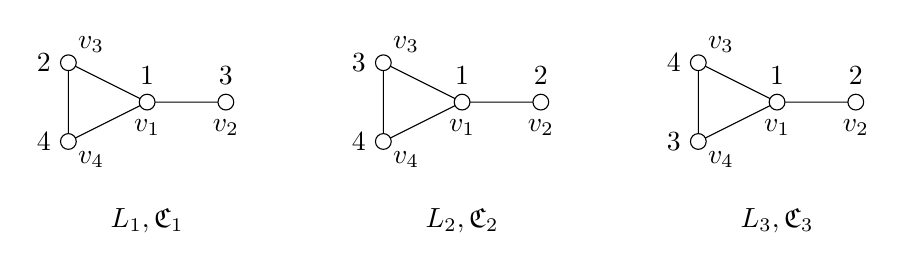
\begin{tikzpicture}
\draw(1,0)--(0,0.5)--(0,-0.5)--(1,0)--(2,0); \draw[fill=white](1,0)circle(0.1); \node[below]at(1,-0.1){$v_1$}; \draw[fill=white](2,0)circle(0.1); \node[below]at(2,-0.1){$v_2$}; \draw[fill=white](0,0.5)circle(0.1); \node[above right]at(0,0.5){$v_3$}; \draw[fill=white](0,-0.5)circle(0.1); \node[below right]at(0,-0.5){$v_4$};
\node[above]at(1,0.1){$1$}; \node[above]at(2,0.1){$3$}; \node[left]at(-0.1,0.5){$2$}; \node[left]at(-0.1,-0.5){$4$}; \node at(1,-1.5){$L_1, \PP_1$};

\begin{scope}[shift={(4,0)}]
\draw(1,0)--(0,0.5)--(0,-0.5)--(1,0)--(2,0); \draw[fill=white](1,0)circle(0.1); \node[below]at(1,-0.1){$v_1$}; \draw[fill=white](2,0)circle(0.1); \node[below]at(2,-0.1){$v_2$}; \draw[fill=white](0,0.5)circle(0.1); \node[above right]at(0,0.5){$v_3$}; \draw[fill=white](0,-0.5)circle(0.1); \node[below right]at(0,-0.5){$v_4$};
\node[above]at(1,0.1){$1$}; \node[above]at(2,0.1){$2$}; \node[left]at(-0.1,0.5){$3$}; \node[left]at(-0.1,-0.5){$4$}; \node at(1,-1.5){$L_2, \PP_2$};
\end{scope}

\begin{scope}[shift={(8,0)}]
\draw(1,0)--(0,0.5)--(0,-0.5)--(1,0)--(2,0); \draw[fill=white](1,0)circle(0.1); \node[below]at(1,-0.1){$v_1$}; \draw[fill=white](2,0)circle(0.1); \node[below]at(2,-0.1){$v_2$}; \draw[fill=white](0,0.5)circle(0.1); \node[above right]at(0,0.5){$v_3$}; \draw[fill=white](0,-0.5)circle(0.1); \node[below right]at(0,-0.5){$v_4$};
\node[above]at(1,0.1){$1$}; \node[above]at(2,0.1){$2$}; \node[left]at(-0.1,0.5){$4$}; \node[left]at(-0.1,-0.5){$3$}; \node at(1,-1.5){$L_3, \PP_3$};
\end{scope}
\end{tikzpicture}\\
\caption{For $i=1,2,3$, a representative labeling $L_i$ associated with the coupling $\PP_i$, as defined in Remark \ref{r:ord4couplings}\label{fig:paw-couple}.}
\end{center}
\end{figure}


\noi\underline{Coupling $\PP_1=
\{(v_1,v_2),(v_3,v_4)\}$ {and labeling $L_1$ shown in Figure \ref{fig:paw-couple}}:} The pendent vertex is labeled $3$.
Then positive definite matrices {$\symp({\rm Paw}^{L_1})$}  have the form 
\[
\left[\begin{array}{rrrr}
a & f & e & g \\
f & c & 0 & h \\
e & 0 & b & 0 \\
g & h & 0 & d
\end{array}\right] {.}
\] 
One can verify that 
\[
(\Omega N)^2= 
\left[\begin{array}{rrrr}
-a b + e^{2} & -b f & 0 & -b g \\
-d f + e g + g h & -c d + h^{2} & b g & 0 \\
0 & e f + c g - f h & -a b + e^{2} & -d f + e g + g h \\
-e f - c g + f h & 0 & -b f & -c d + h^{2}
\end{array}\right] {.}
\] 
In particular, the $(1,4)$-entry is nonzero. 
Hence $(\Omega N)^2 +tI \neq O$ for each $t$.  Hence every positive definite matrix 
with this partitioned graph has distinct symplectic eigenvalues.
\bigskip



\noi\underline{Coupling $\PP_2=\{(v_1,v_3),(v_2,v_4)\}$ {and labeling $L_2$ shown in Figure \ref{fig:paw-couple}}:} 
The pendant vertex  is labeled 2. 
 The leading principal minors of
\[ 
 N=
\left[ \begin{array}{rrrr}
 3 &-1 &  1&  1 \\
-1 &  1 &  0&   0 \\
1 &  0&  1 & 1\\
 1 & 0 & 1 & 2
 \end{array} \right].
\] 
 equal 3, 2, 1 and 1{, so} 
$N$ is positive definite.  
Also, one can verify that  $(\Omega N)^2=-I$. Hence, the symplectic eigenvalues of $N$ each equal $1$. 
 {Since $\G^L(N)={\rm Paw}^{L_2}$,} this labeled  Paw graph is symplectic spectrally arbitrary.

Additionally, $N$ has the SSSP.  To see this, 
note that if $Y$ is a matrix of the form
\[ \left[\begin{array}{rrrr}
0 & 0 & 0 & 0 \\
0 & 0 & a & b \\
0 & a & 0 & 0 \\
0 & b & 0 & 0
\end{array}\right] 
\]
such that 
$\Omega NY= YN\Omega$, then 
\[ \left[\begin{array}{rrrr}
0 & a + b & 0 & 0 \\
a + b & 2 \, a + 4 \, b & -a - b & 0 \\
0 & -a - b & 2 \, a & -a + b \\
0 & 0 & -a + b & -2 \, b
\end{array}\right]=O.\]
This occurs only if $Y=O$, and hence $N$ has the SSSP.  
\end{ex}

\begin{ex}\label{K22cup2}
 Name the vertices of $K_{2,2}$ so that the partite sets are $\{v_1,v_2\}$ and  $\{v_3,v_4\}$. Then $\PP_2$ is covered by the labeled graph $K_{2,2}^M$, which was shown to allow a sympPD matrix {with the SSSP} in Example \ref{KppSympPD-SSSP} and by  symmetry the coupling $\PP_3$ is covered.   


For the coupling $\PP_1=\{(v_1,v_2),(v_3,v_4)\}$, consider the matrix
\begin{align}
\label{eq:PP2}
 N=
 \mtx{
 \begin{array}{rrrr}
2 & 1 & 0 & 1 \\
 1 & 2 & 1 & 0 \\
 0 & 1 & 2 & -1 \\
 1 & 0 & -1 & 2 
 \end{array}
 }.
\end{align} 
The (standard) eigenvalues of $N$ are $2+\sqrt 2, 2+\sqrt 2,2-\sqrt 2,2-\sqrt 2$, so  $N$ is positive definite.
Also, one can verify that $(\Omega N)^2=-2I$, so $\spspec(N)=\{\sqrt 2,\sqrt 2\}$.
  Thus this labeling of $K_{2,2}$ is symplectic spectrally arbitrary. Note that the labeling used here is that of $C_4^I$  in Example \ref{ex:verify-cycle}, where it is shown that every  matrix of this form  has the SSSP ($C_4^I$  and $K_{2,2}^M$ are  different labelings of the same graph),   and hence all labelings of $C_4\cong K_{2,2}$ are  symplectic spectrally arbitrary and for each labeling there is a sympPD matrix with the SSSP. 
\end{ex}

\begin{ex}\label{K4-ecup2}
Name the vertices of $\OL{K_2}\vee K_2$ so that  $v_1$ and $v_2$ are not adjacent.
 Then $\PP_2$ is covered by the labeled graph $(\OL{K_2}\vee K_2)^M$ and by  symmetry the coupling $\PP_3$ is covered.  
For the coupling $\PP_1=\{(v_1,v_2),(v_3,v_4)\}$, we use the labeling $L(v_1)=1, L(v_2)=3, L(v_3)=2, L(v_4)=4$ and observe that  $(\OL{K_2}\vee K_2)^L$ is a supergraph of $C_4^I$.  Since  a sympPD matrix $N\in\symp(C_4^I)$ with the SSSP was exhibited in Example \ref{K22cup2}, Theorem \ref{supergraph} implies that $(\OL{K_2}\vee K_2)^L$ allows a sympPD matrix and is therefore symplectic spectrally arbitrary.  \end{ex}
\ms


  Next we consider the five unlabeled disconnected graphs of order four: $4K_1$, $2K_1\du K_2$, $2K_2$, $K_1\du P_3$, and $K_1\du K_3$.
The graph $4K_1$ is  clearly symplectic spectrally arbitrary. The graphs $K_1\du P_3$ and $K_1\du K_3$ must have all simple symplectic eigenvalues by Proposition \ref{iso-isol}.
For the remaining two disconnected graphs of order four, we consider the coupling. Let $\GC G C$ be a coupled graph with subgraph $H$.   The coupling \emph{respects $H$} if $\pp(v)\in H$ for every $v\in V(H)$; in this case, the \emph{coupling $\PP$ restricted to $H$} is the coupling $\PP|_{H}$ of $H$ where $\pp|_{H}(v)=\pp(v)$.  We first develop a matrix tool.









 \begin{thm}
\label{directsum}
Let $P$ and $Q$ be  $2m \times 2m$ 
and $2r \times 2r$  positive definite matrices
with block forms
$
P=\left[ \begin{array}{cc}
P_1  & P_2 \\ 
P_2\trans & P_3 \end{array} \right]$,
$Q=\left[ \begin{array}{cc}
Q_1  & Q_2 \\ 
Q_2\trans & Q_3 \end{array} \right]$
where $P_1$ is $m\times m$ (respectively, $Q_1$ is 
$r \times r$), 
and let 
\[ N=\left[ 
\begin{array}{cccc}
P_1 & O & P_2 & O \\  
O & Q_1 & O & Q_2 \\ 
P_2\trans & O &P_3 & O \\  
O & Q_2\trans & O & Q_3
\end{array} \right]. 
\] 
Then: 
\ben[$(a)$]
\item 
\label{directsum-a}
$N$ is positive definite.
\item
\label{directsum-b}$
\spspec(N)=\spspec(P) \cup \spspec(Q)$.
\item
\label{directsum-c}
If $P$ and $Q$ have the SSSP and  $\spspec(P) \cap \spspec(Q)= \emptyset$, then $N$ has the SSSP. 
\een
\end{thm}


\begin{proof} 
Since $N$ is permutationally similar to $P\oplus Q$, \eqref{directsum-a} holds. 

Let $p=m+r$, 
\[R= \mtx{
I_m & O & O & O \\ 
O & O & I_r & O \\  
O & I_m & O & O \\ 
O & O & O & I_r
} \!\!, \ \widehat{\Omega}= R\trans \Omega R, \  \mbox{and} \ \widehat{N}= R\trans N R.\] 
Then 
\beq \label{eq1} \widehat{\Omega}=
\Omega_m \oplus \Omega_r \ \mbox{ and }\  \widehat{N}= P \oplus Q .\eeq 
Since $R$ is a permutation matrix,  
\[ \spec(\Omega N)=\spec(R\trans \Omega N R)=\spec(\wh \Omega \wh N) =\spec((\Omega_m P)\oplus ( \Omega_r Q))=\spec(\Omega_m P)\cup \spec(\Omega_r Q).\]
Therefore, \eqref{directsum-b} holds. 


Now assume that both $P$ and $Q$ have the SSSP, and let $Y$ be a symmetric  $p\x p$ matrix such that $N \circ Y=O$
and  $\Omega N Y = Y N \Omega$.
Let 
\[\widehat{Y} = R\trans Y R = \mtx{\widehat{Y}_{11} & \widehat{Y}_{12} \\ 
{\widehat{Y}_{12}}\trans & \widehat{Y}_{22}}
\]
where $\wh Y_{11}$ is $m\x m$ and $\wh Y_{22}$ is $r\x r$.  Evidently, 
\begin{eqnarray}
\label{eq3}
 \widehat{\Omega} \widehat{N}\widehat{Y}&=&\widehat{Y}\widehat{N}\widehat{\Omega}, \mbox{ and }
\\
\label{eq4} 
\widehat{N} \circ \widehat{Y}& =&O.
\end{eqnarray} 


Equations \eqref{eq1} and \eqref{eq3} imply that 
\begin{eqnarray}
\label{eq5}
\Omega_m P\widehat{Y}_{11} &=& 
\widehat{Y}_{11}P\Omega_m, \\
\label{eq6}
\Omega_r Q\widehat{Y}_{22}  &= &  
\widehat{Y}_{22}Q\Omega_r, \mbox{ and }\\
\label{eq7} 
 \Omega_m P \widehat{Y}_{12} & = &  \widehat{Y}_{12} Q \Omega_r  
\end{eqnarray}

By (\ref{eq4}), (\ref{eq5}), and the fact $P$ has the SSSP, 
$\widehat{Y}_{11}=O$.  Similarly, 
$\widehat{Y}_{22}=O$.  Equation (\ref{eq7}) 
implies that $(\Omega_m P) \widehat{Y}_{12}  -  \widehat{Y}_{12} (Q \Omega_r)=O$.
  Since $P$ and $Q$ have no common symplectic eigenvalue, $\spec(\Omega_m P)\cap \spec(\Omega_r Q)=\emptyset$, and $\spec(Q \Omega_r)=\spec( \Omega_r Q)$.
Then Sylvester's Theorem (see, e.g.,  \cite[Theorem 2.4.4.1]{HJ}) implies $\widehat{Y}_{12}=O$. Hence $\widehat{Y}=O$, and $Y=O$. By Theorem \ref{SSSPequiv}, \eqref{directsum-c} holds.
\end{proof} 


 Let $\GC G C$ be  a coupled  graph of order $n=2p$. For a multiset $\LS$
of $p$ positive real numbers, we say $\GC G C$ \emph{allows the symplectic spectrum $\LS$} (respectively, \emph{allows the symplectic spectrum $\LS$ with the SSSP})  if there is a representative labeling $L$ for $\GC G C$ and a matrix $N\in\symp(G^L)$ such that $\spspec(N)=\LS$ (respectively,  $\spspec(N)=\LS$ and $N$ has the SSSP). We also apply similar terminology to a graph and standard spectrum, e.g., $G$ \emph{allows the  spectrum $\Lambda$}   if there is  a matrix $A\in\symm(G)$ such that $\spec(A)=\Lambda$.


\begin{cor}\label{symplectic_disj_union}  Let $\GC G C$ be a coupled graph, let  $G_1$ be a subgraph respected by $\PP$, and let $G_2$ be the subgraph of $G$ induced by the complement  of $V(G_1)$.  Denote the order of $G$ by $2p$ and the order of $G_1$ by $2m$, and let $r=p-m$.
\ben[$(a)$]
\item\label{Ssubgarph1}   If $G=G_1\du G_2$ (i.e., there are no edges between $G_1$ and $G_2$) and $G_i^{\PP|_{G_i}}$ allows symplectic spectrum $\LS_i$ for $i=1,2$, then $\GC G C$ allows the symplectic spectrum $\LS_1\cup\LS_2$. 

If $m=r=1$ and $G=G_1\du G_2$, then $G$ allows all symplectic eigenvalues equal, and so is symplectic spectrally arbitrary.

\item \label{Ssubgarph2}  If  $G_1^{\PP|_{G_1}}$ allows symplectic spectrum $\LS_1$ with the SSSP, then $\GC G C$ allows allows the symplectic spectrum $\LS_1\cup \{d_1,\dots,d_r\}$ with SSSP for any distinct positive real numbers $d_i, i=1,\dots,r$ such that $d_i\not\in\LS_1$ for $i=1,\dots,r$.
\een 
  \end{cor}
\bpf Choose   a representative labeling $L$  of $\PP$ such that  $G_1$ is labeled by  $\alpha_1=\{1,\dots,m\}\cup\{p+1,\dots,p+m\}$.  Observe that $\PP$ respects $G_2$ and  that  $G_2$ is labeled by $\alpha_2=\{m+1,\dots,m+r\}\cup\{p+m+1,\dots,2p\}$.
Let $L_i$ denote the labeling $L$ restricted to $G_i$. 

\eqref{Ssubgarph1}: Assume the hypotheses.   
Choose $N_i\in\symp(G_i^{L_i})$ with $\spspec(N_i)=\LS_i$ and define $N\in\symp(G^L)$ such that $N[\alpha_i]=N_i$ and all other entries are zero.  Then \[\spspec(N)=\spspec(N_1)\cup\spspec(N_2)=\LS_1\cup\LS_2\] by Theorem \ref{directsum}.  The second statement is immediate from the first statement and Remark \ref{o4sympPD3SSA}.

\eqref{Ssubgarph2}: Assume $G_1^{\PP|_{G_1}}$ allows symplectic spectrum $\LS_1$ with the SSSP and let  $d_1,\dots,d_r$ be distinct positive real numbers such that $d_i\not\in\LS_1$ for $i=1,\dots,r$. 
Choose $N_1\in\symp(G_1^{L_1})$ with $\spspec(N_1)=\LS_1$ and let $D$ be an $r\x r$ matrix with diagonal entries $d_1,\dots,d_r$.
Define $N\in\symp(G^L)$ such that $N[\alpha_1]=N_1$, $N[\alpha_2]=D$ and all other entries are zero. Then $\spspec(N)=\LS_1\cup \{d_1,\dots,d_r\}$ and $N$ has the SSSP by Theorem \ref{directsum}. 
\epf


Corollary \ref{symplectic_disj_union}
\eqref{Ssubgarph1} 
can be used to study certain labeled graphs 
that are  disjoint unions of labeled graphs. 

\begin{ex}\label{ex:2K1K2}
    Consider the graph $2K_1\du K_2$ where the isolated vertices are named $v_1$ and $v_3$ and the vertices of $K_2$ are named $v_2$ and $v_4$.  By graph symmetry, we need consider only two couplings, $\PP_2=\{(v_1,v_3), (v_2,v_4)\}$, which respects $2K_1$ and $K_2$, and a coupling such as $\PP_1=\{(v_1,v_2), (v_3,v_4)\}$ where an isolated vertex is coupled with a vertex of $K_2$.
     By Corollary \ref{symplectic_disj_union}\eqref{Ssubgarph1}, $G^{\PP_2}$ allows all symplectic spectra, so  every labeling $L$ associated with $\PP_2$, the labeled graph $(2K_1\du K_2)^L$ is symplectic spectrally arbitrary. A labeling associated with $\PP_1$ requires simple symplectic eigenvalues by Proposition \ref{iso-isol}.
\end{ex}



\begin{ex}\label{ex:2K2}
    Consider the graph $2K_2$ where the the vertices of one $K_2$ are named $v_1$ and $v_3$ and of the other $K_2$ are named $v_2$ and $v_4$.  By graph symmetry, we need consider only two couplings, $\PP_2=\{(v_1,v_3), (v_2,v_4)\}$, which respects $K_2$ and $K_2$, and a coupling such as $\PP_1=\{(v_1,v_2), (v_3,v_4)\}$ where a vertex of one $K_2$ is coupled with a vertex of the other $K_2$.
For every labeling $L$ associated with $\PP_2$, $(K_2\du K_2)^L$  is symplectic spectrally arbitrary by Corollary \ref{symplectic_disj_union}\eqref{Ssubgarph1}.

 Now consider the coupling $\PP_1=\{(v_1,v_2), (v_3,v_4)\}$ with labeling $L$ defined by {$L(v_1)= 1,  L(v_2)= 3, L(v_3)= 2,L(v_4)=4$}.  
 This is $(K_2\du K_2)^I$, which is symplectic spectrally arbitrary by Example \ref{random}.
 So every labeling of $K_2\du K_2$ is symplectic spectrally arbitrary.
\end{ex}

 The two previous examples complete the solution to the ISEP-$G$ for graphs of order four.
Corollary \ref{symplectic_disj_union}
\eqref{Ssubgarph2} can be used to show to provide forbidden families of labeled subgraphs for certain symplectic spectral properties. 

\begin{ex}
\label{ex:P6}
Consider the matrix 
\[ 
N=
\renewcommand{\arraystretch}{1.25}
\left[\begin{array}{rrrrrr}
1 & \frac{1}{2} & 0 & 0 & 0 & 0 \\
\frac{1}{2} & \frac{5}{4} & \frac{1}{2} & 0 & 0 & 0 \\
0 & \frac{1}{2} & \frac{24}{25} & \frac{1}{10} & 0 & 0 \\
0 & 0 & \frac{1}{10} & 1 & -\frac{1}{2} & 0 \\
0 & 0 & 0 & -\frac{1}{2} & \frac{5}{4} & -\frac{1}{2} \\
0 & 0 & 0 & 0 & -\frac{1}{2} & 1
\end{array}\right].
\]
{Let $\II$ denote a coupling of a path graph such that labeling the vertices  in path order is a representative labeling, so the coupled graph  of $N$ is $P_6^\II$.} 
The determinants of the leading principal submatrices of $N$ are
each positive; namely, they are
$1$, $1$, $71/100$, $7/10$,
$279/400$ and $209/400$.
Hence $N$ is positive semidefinite. 
The matrix 
\[
\Omega N=
\renewcommand{\arraystretch}{1.25}
\left[\begin{array}{rrrrrr}
0 & 0 & \frac{1}{10} & 1 & -\frac{1}{2} & 0 \\
0 & 0 & 0 & -\frac{1}{2} & \frac{5}{4} & -\frac{1}{2} \\
0 & 0 & 0 & 0 & -\frac{1}{2} & 1 \\
-1 & -\frac{1}{2} & 0 & 0 & 0 & 0 \\
-\frac{1}{2} & -\frac{5}{4} & -\frac{1}{2} & 0 & 0 & 0 \\
0 & -\frac{1}{2} & -\frac{24}{25} & -\frac{1}{10} & 0 & 0
\end{array}\right]
\] 
 has characteristic polynomial $(x^2 + 209/400)(x^2 + 1)^2$.
Hence $N$ has symplectic eigenvalues $1$, $1$, and
 $\sqrt{209/400}$. In particular, $N$ has a multiple symplectic eigenvalue.
A direct computation shows that $N$ has the SSSP. 
\end{ex}  

The following is a consequence of Corollary \ref{symplectic_disj_union}
\eqref{Ssubgarph1}, 
Example \ref{ex:paw}, Example \ref{ex:P6}, Example \ref{K22cup2}, and Example \ref{random}.






\begin{thm}\label{forbid4simple}
 Let $\GC G C$ be a coupled graph on $2p$ vertices such that 
 $G_1$ is a subgraph respected by $\PP$ on $2k$ vertices. 
 If $G_1$ is any of the following, then there is a positive definite matrix
  with labeled graph  representing $\GC GC$ with a non-simple symplectic eigenvalue: 

\ben[\rm $(a)$]
\item A paw whose pendent edge does not join a vertex $v$ with $\mathfrak{c}({v})$.
\item $P_6^{\II}$.
\item A $4$-cycle.
\item A complete graph of order at least four.
\een 
\end{thm}

%%%%%%%%%%%%%%%%%%%%%%%%%%%%%%%%%%%%%%%%%

\section{Coupled Zero Forcing}
\label{s:zeroforcing}

 Zero forcing and its variants such as positive definite and skew zero forcing  provide well-known  combinatorial upper bounds for the 
maximum nullities of the relevant types of  matrices described by  {a} graph, beginning with standard zero forcing  and {maximum nullity, or equivalently, maximum eigenvalue multiplicity for the standard} IEP-$G$ \cite{AIM08}  
(see  \cite[Chapter 9]{HLSbook} for discussion of variants).   In this section we define a new form of zero forcing for coupled graphs as an upper bound on the maximum multiplicity of a symplectic eigenvalue among matrices associated with the coupled graph.  We use coupled zero forcing and prior results to solve the ISEP-$G$ for several families of graphs. We also characterize coupled graphs that have coupled zero forcing number equal to one.


We begin by recalling the definition of the standard maximum nullity  and defining the maximum symplectic eigenvalue multiplicity   for a coupled graph.
Let $G$ be an unlabeled graph. The \emph{standard maximum nullity} of $G$ is $\M(G)=\max\{\null A \colon A\in\symm(G)\}$.
Since the nullity of $A-\lam I$ is the multiplicity of $\lam$ as an eigenvalue of $A$ and $\G(A-\lam I)=\G(A)$, $\M(G)$ is the maximum multiplicity of an eigenvalue of $A\in\symm(G)$.





\begin{defn}[Maximum symplectic multiplicity]
    Let $\GC G C$ be a coupled graph  and let $L$ be a representative labeling of $\GC G C$.  The \emph{maximum symplectic multiplicity of $\GC G C$}, denoted by $\MC(\GC G C )$, is the maximum multiplicity among the symplectic eigenvalues of matrices $N\in\symp(G^L)$. 
\end{defn}

Next we recall the definition of the standard zero forcing number and define the coupled zero forcing color change rule and number. Let $G$ be an unlabeled graph. The \emph{standard color change   rule} allows a blue vertex $v$ to force a white vertex $w$ to blue if $w$ is the only white vertex in $N(v)$. 
A set $B\subseteq V(G)$ of initially blue vertices is called a \emph{standard zero forcing set} of $G$ if repeated application of the standard zero forcing color change rule eventually colors every vertex of $G$ blue. The \emph{standard zero forcing number} of $G$, denoted by $\Z(G)$, is the minimum cardinality of a standard zero forcing set of $G$. 


\begin{defn}[Coupled zero forcing] 
Let $\GC G C$ be a coupled graph, and suppose each vertex is colored either blue or white. The \emph{coupled zero forcing color change rule} consists of the following two operations:
\begin{enumerate}
    \item A blue vertex $v$ forces a white vertex $w$ to blue, denoted $v\to w$, if $w$ is the only white vertex in $N(v)\cup \{\pp(v)\}$.
    \item A white vertex $v$ forces itself to blue, denoted $v\to v$, if every vertex in $N(v)\cup \{\pp(v)\}$ is blue. 
\end{enumerate}
 A subset of  $V(G)$ of initially blue vertices is called a \emph{coupled zero forcing set} of $\GC G C$ if repeated application of the coupled zero forcing color change rule eventually colors every vertex of $\GC G C$ blue. It follows from known results about $\Z_\ell$ (see Remark \ref{ZCZell}) that the final coloring of a coupled zero forcing set is independent of the forces chosen. The \emph{coupled zero forcing number} of $\GC G C$, denoted by $\ZC(\GC G C)$, is the minimum cardinality of a coupled zero forcing set of $\GC G C$. 
\end{defn}


   The proof that $\ZC(\GC G C)$ provides an upper bound for $\MC(\GC G C)$   is  in some ways similar to the same relation between the standard zero forcing number and the maximum multiplicity, but there is also a fundamental difference, which is discussed in the remark following the proof. 


\begin{thm}\label{prop_zer_forc_vs_mult}
    Let $\GC G C$ be a coupled graph. Then $\MC(\GC G C) \leq \ZC(\GC G C)$.
\end{thm}
\begin{proof} 
    Let $N$ be a real positive definite matrix whose  labeled graph  is a representative labeling of $\GC G C$, and let $B$ be any coupled zero forcing set of $\GC G C$. 
    Suppose $\mu$ is an eigenvalue of $\Omega N$ with eigenvector $\bx=[x_i]$ such that $x_k = 0$ for all $k\in B$. 
     Since $(\mu I - \Omega N) \bx = 0$, multiplying on the left by $\Omega$ and using $\Omega^2 = -I$ yields $(\mu \Omega + N)\bx = 0$. Set $N' = \mu \Omega + N$ and $N'=[n'_{ij}]$; hence $\bx \in \ker(N')$. 
    Notice that, for every   vertex  label $v$, $n'_{vv} \neq 0$ and $n'_{v,\pp(v)} \neq 0$ since $N$ is a real positive definite matrix and  $\mu$ is a  nonzero  purely imaginary number.  Because an application of the coupled zero forcing color change rule corresponds to showing another entry in the null vector $\bx$ is zero, repeated application shows that  $\bx$ is the zero vector.  Thus, the kernel of $\mu I- \Omega N$ does not contain a nonzero vector with $x_k=0$ for all $k\in B$. Hence, the  multiplicity of $\mu$ as an eigenvalue of $\Omega N$ is at most $|B|$
    (see Lemma 2.13 of \cite{HLSbook}).   Since $\Omega N$ is real, its purely imaginary eigenvalues occur in complex conjugate pairs. Thus, by Proposition \ref{sympev}, the multiplicity of $\mu$ as an eigenvalue of $\Omega N$  equals the multiplicity of the symplectic eigenvalue $|\mu|$ of $N$. Since $\mu$ and $N$ are arbitrary, we have 
     $\MC(\GC G C) \leq \ZC(\GC G C)$. 
\end{proof}


\begin{rem}
    Note that  the proof given above is specific to the real numbers, because it relies on the fact that the sum of a real number and a nonzero purely imaginary number is necessarily nonzero. This is different from   the situation with standard maximum nullity and zero forcing, where $\M^F(G)\le\Z(G)$ regardless of the field $F$ in which the matrices reside,
    (whether $\M^F(G)$ can be interpreted as the maximum multiplicity of an eigenvalue rather than as maximum nullity {may}  vary with field, as {may}   the value of $\M^F(G)$ for a fixed graph $G$.)
\end{rem}




\begin{ex}\label{example_path_simple}
    Let us consider the path graph $P_{2p}$ with vertices  named  in path order, i.e., $v_j$ is adjacent to  $v_{j+1}$ for all $j \in \{1,\ldots,2p-1\}$. Consider the coupling ${\MM}= \{(v_1,v_2),(v_3,v_4),\ldots,$ $ (v_{2p-1},v_{2p})\}$. Then it is easy to see that $\{v_1\}$ is a coupled zero forcing set, and hence $\ZC(P_{2p}^{\MM}) = 1$. Theorem \ref{prop_zer_forc_vs_mult} implies that $\MC(P_{2p}^{\MM}) = 1$. Therefore, the path graph $P_{2p}$ with coupling $\MM$ requires all  symplectic eigenvalues to be simple. 
\end{ex}


In fact, coupled zero forcing on $G^\PP$ can be viewed as loop zero forcing on a graph $G(\PP)$ defined from $G$ and $\PP$. The {\em  loop zero forcing number} of a (simple unlabeled) graph $G$,  denoted by $\Zell(G)$, is  the zero forcing number defined by the $\Zell$-color change rule \cite{param}:
\ben\item If $u$ is blue and exactly one  neighbor $w$ of $u$  is white, then change the color of $w$ to blue.  
\item If $w$ is white,  $w$ is not an isolated vertex, and every neighbor of $w$ is blue, then change the color of $w$ to blue.
\een


\begin{defn}
Given a coupled graph $\GC G C$, define the simple unlabeled graph $G(\PP)$ by starting with $G$  and  adding an edge (if not already present) between $v$ and $\pp(v)$ for each pair of coupled vertices. 
\end{defn}
  
Observe that for any coupled graph $\GC G C$, the graph $G(\PP)$ always contains a perfect matching defined by the coupling, i.e., the edges  with endpoints $v$ and $\pp(v)$.   If $G$ has a perfect matching $M$, then $M$ naturally defines a coupling, called the \emph{coupling defined by $M$} and denoted by $\MM$, by choosing the pairs of endpoints of the edges in the matching  as the coupling.

\begin{rem}\label{ZCZell} {Since  $G(\PP)$  contains a perfect matching, it}  has no isolated vertices. Thus applying the coupled zero forcing color change rule to $\GC G C$ is  the same as applying the $\Zell$-color change rule to $G(\PP).$
    In particular, if $v$ and $\pp(v)$ are already adjacent in $G$ for every vertex $v$, then $G(\PP)=G$ { and $\Z_{C}(G)=\Zell(G)$}. 
\end{rem}

\begin{obs}\label{obs-delta-Zell}
    It is immediate from the definition that $\delta(G)\le \Zell(G) {\le \Z(G)}$.  { If $v$ and $\pp(v)$ are already adjacent in $G$ for every vertex $v$, then  $\delta(G) \le  \Z_{C}(G)\le \Z(G)$.}
\end{obs}

\begin{ex} 
    Let us consider the  cycle graph $C_{2p}$  with vertex names  in cycle order, i.e., $v_j$ is adjacent to $v_{j+1}$ for all $j \in \{1,\ldots,2p-1\}$ and $v_{2p}$ is adjacent to $v_1$. 
    Consider the coupling ${ \MM}=\{(v_1,v_2),(v_3,v_4),\ldots,(v_{2p-1},v_{2p})\}$.  Then  $C_{2p}(\MM)= C_{2p}$ and $2=\delta(C_{2p})\le \ZC (C_{2p}^{\MM}) =\Zell(C_{2p})\le \Z(C_{2p})= 2$, 
    and Theorem \ref{prop_zer_forc_vs_mult} implies that $ \MC(C_{2p}^\MM) \leq 2$. 
\end{ex}

   Next we apply coupled zero forcing to solve the ISEP-$G$ for some additional families of graphs.  The \emph{corona} of $H$ with $K_1$, denoted by $H\circ K_1$, is formed from a graph $H$ by joining a new vertex $u_v$ to $v$ for each vertex $v$ of $H$.    We begin by developing some additional tools for graphs of the form $H\circ K_1$.
Let $H$ be a graph of order $p$.  Observe that $H\circ K_1$ has a unique perfect matching in which each leaf $u_v$ is matched with its neighbor $v\in V(H)$. Let $M$ be a representative labeling of the coupling $\MM$ defined by the perfect matching in which the leaves $G$ are labeled $1,\dots,p$. 


\begin{lem}\label{HcircK1}
     Let $H$ be a graph of order $p$ and let $\GC G M=(H\circ K_1)^{\MM}$. Then: 
     \ben[$(a)$]
     \item\label{HcircK1Z}   $\ZC(\GC G M)=\Zell(G)\le \Z(H)$.
     \item\label{HcircK1N}
    $N=\mtx{D & E\\E & A}\in \symp(G^{M})$ if and only if
    $
    A\in\sym(H^{M})$ {where $H^M$ has the labeling induced by the labeling of $G^M$}, $D$ and $E$ are diagonal matrices, $D$ is positive definite  and each standard eigenvalue of $\sqrt{D}A\sqrt{D}-E^2$
     is a positive real. 
    In this case, $\spspec(N)=\{\sqrt{\lam_1},\dots,\sqrt{\lam_p}\}$ where $\spec (\sqrt{D}A\sqrt{D}-E^2)=\{\lam_1,\dots,\lam_p\}$; note $\sqrt{D}A\sqrt{D} -E^2\in   \sym(H^M)$. 
   
    \item \label{HcircK1oml} If  $H$ allows  every standard spectrum with ordered multiplicity list $\oml$, then  the coupled graph $\GC G M=(H\circ K_1)^{\MM}$ allows  every symplectic spectrum with ordered multiplicity list $\oml$.\een
\end{lem}
\bpf
\eqref{HcircK1Z}: From the definition of $\MM$, we see that $G(\MM)=G$, so $\ZC(\GC G M)=\Zell(G)$. Any standard zero forcing set for $H$ is   a $\Zell$-forcing set for $G$, so $\Zell(G)\le \Z(H)$.

\eqref{HcircK1N}: 
Let $N=\mtx{D & E\\E & A}$ be a  symmetric matrix  where $D$ and $E$ are  $p\times p$ diagonal matrices, and $A$ is a symmetric $p\x p$ matrix. It is immediate that 
$\G^{L}(N)=(H\circ K_1)^{M}$ if and only if $\G^L(A)=H^{M}$, and that if $N$ is positive definite 
then so is $D$. So we may assume that $D$ is positive definite and $\G^L(A)=H^{M}$.

Note that
$S=\begin{bmatrix}
D^{-1/2} &-D^{-1/2}E \\
O & D^{1/2} 
\end{bmatrix}
$
is  symplectic and 
$S\trans NS =\begin{bmatrix}
I  & O_p\\
O_p & \sqrt{D}A\sqrt{D}-E^2
\end{bmatrix}.$ 
Thus $N$ is positive definite if and only if each (standard) eigenvalue of $\sqrt{D}A\sqrt{D}-E^2$ is a positive real,  and 
in this case $\spspec(N)=\spspec(S\trans N S)$.

We now assume that $N$ is positive definite, 
and compute $\spspec{(S\trans NS)}$ by determining 
the (standard) spectrum of  $\Omega_{2p} S\trans NS$.
Note that 
\begin{align*}
\det(xI_{2p}-\Omega_{2p}S\trans NS )
&= \det \begin{bmatrix} xI_p & -\sqrt{D}A\sqrt{D} +E^2 \\
I & xI_p \end{bmatrix}\\
&=
\det\lp x^2I_p+(\sqrt{D}A\sqrt{D} -E^2)\rp.\end{align*}
Hence, the symplectic eigenvalues of $S\trans NS$ (and hence of $N$) are $ \lambda_i\sqrt{-1}$ where 
$\lambda_1, \ldots, \lambda_p$ are the standard eigenvalues of $\sqrt{D}A\sqrt{D} -E^2$.


\eqref{HcircK1oml}: Assume $H$ allows  every standard spectrum with ordered multiplicity list $\oml =(m_1,\dots,m_q)$. Given  positive real numbers $\nu_1<\dots<\nu_q$,  we can choose a matrix $A\in \sym(H)$ such that  the (standard) eigenvalues of $A$ are $\nu_i^2+1$ with multiplicity $m_i$ for $i=1,\dots,q$.  For $N=\mtx{I & I\\I & A}\in \symp(G^{M})$,  the symplectic eigenvalues of $N$ are  $\nu_i$ with multiplicity $m_i$ for $i=1,\dots,q$. by \eqref{HcircK1N}. 
\epf


\begin{prop}
\label{HcircK1MZ}
    Let $H$ be a graph  that  allows  every standard spectrum with multiplicity at most $\M(H)$. Then the coupled graph $\GC G M=(H\circ K_1)^{\MM}$ allows  every symplectic spectrum with multiplicity at most $\M(H)$.
    If in addition $\M(H)=\Z(H)$, then\[\M(H)=\MC(G^{\MM})=\ZC(G^{\MM})=\Zell(G)=\Z(H).\]
\end{prop}
\bpf 
Since $H$ allows every ordered multiplicity list such that the maximum multiplicity is at most $\M(H)$, the first statement follows from Lemma \ref{HcircK1}\eqref{HcircK1oml}.  
This implies $\MC(G^{\MM})\ge \M(H)$. Since  $\MC(G^{\MM})\le \ZC(G^{\MM})$ by Theorem \ref{prop_zer_forc_vs_mult} and $\ZC(G^{\MM})=\Zell(G)\le \Z(H)$  by Lemma \ref{HcircK1}\eqref{HcircK1Z},  the hypothesis $\M(H)=\Z(H)$ completes the proof.
\epf




The solutions to  the ISEP-$G$ for graphs of the form  $P_p\circ K_1$ (called  \emph{combs}) and for graphs of the form  $K_p\circ K_1$  are now immediate from Proposition \ref{HcircK1MZ} and the following well-known facts: A path order $p$ allows as a spectrum every set of $p$ distinct real numbers (see \cite{Hochstadt67a} or \cite[Theorem 1.15]{HLSbook}).
The complete graph $K_p$ allows as a spectrum every multi-set of $p$ real numbers that contains at least two distinct numbers  (see \cite{BLMNSSSY13} or \cite[Proposition 1.11]{HLSbook}).  


\begin{cor}\label{PpcircK1}
     The coupled graph $(P_p\circ K_1)^{\MM}$ allows  every distinct symplectic spectrum and does not allow a multiple symplectic eigenvalue.  Furthermore, $\M(P_p)=\MC((P_p\circ K_1)^{\MM})=\ZC((P_p\circ K_1)^{\MM})=\Zell(P_p\circ K_1)=\Z(P_p)=1$.
\end{cor}


\begin{cor}\label{KpcircK1}
     The coupled graph $(K_p\circ K_1)^{\MM}$ allows  every symplectic spectrum with at least two distinct symplectic eigenvalues and does not allow a sympPD matrix.  Furthermore, $\M(K_p)=\MC((K_p\circ K_1)^{\MM})=\ZC((K_p\circ K_1)^{\MM})=\Zell(K_p\circ K_1)=\Z(K_p)=p-1$.
\end{cor}


\begin{thm}{\rm \cite{Ferg80, FF09}} A multiset of real numbers $\lambda_1\le \lambda_2\le \dots\le \lambda_n$ is the spectrum of an $n\x n$  matrix  $A\in\symm(C_n)$  
if and only if
one of the following two conditions holds:
\ben[$(a)$]
\item  $\lambda_{n}>\lambda_{n-1}\ge \lambda_{n-2} > \lambda_{n-3} \ge\cdots $. 
\item $\lambda_{n}\ge \lambda_{n-1}> \lambda_{n-2} \ge \lambda_{n-3} >\cdots $.
\een
\end{thm}

To align with the results we wish to apply, we restate the previous theorem in terms of ordered multiplicity lists.



\begin{cor}  For a strictly increasing ordered set $\Lambda$ of $q$ real numbers  and 
 ordered multiplicity list $\oml=(m_1,\dots,m_q)$ where each $m_i$ equals one or two
 and  $n=\sum_{i=1}^q m_i$,  there exists $A\in\symm(C_n)$ with $\spec(A)=\Lambda$ if and only if $\sum_{i=k}^{k'}m_i$ is even
 for any $1\leq k< k'\leq q$ such that $m_k=m_{k'}=2$.
 
\end{cor}

\begin{cor}\label{CpcircK1}
The coupled graph $(C_p\circ K_1)^{\MM}$ allows  every symplectic spectrum that can be described by an 
 ordered multiplicity list $\oml=(m_1,\dots,m_q)$  where each $m_i$ equals one or two,
 $p=\sum_{i=1}^q m_i$, and
   $\sum_{i=k}^{k'}m_i$ is even for any $1\leq k< k'\leq q$ such that $m_k=m_{k'}=2$. No other symplectic spectra are allowd.
 Furthermore, $\M(C_p)=\MC((C_p\circ K_1)^{\MM})=\ZC((C_p\circ K_1)^{\MM})=\Zell(C_p\circ K_1)=\Z(C_p)=2$.
 \end{cor} 



Corollaries \ref{PpcircK1}, \ref{KpcircK1} and \ref{CpcircK1} are only specific examples of a more general situation, described next. 

\begin{rem}\label{r:HcircK1}  Let $H$ is a graph for which the IEP-$G$ is solved
 by specifying which ordered multiplicity lists are permitted and all spectra are allowed for these lists.  Then  the ISEP-$G$ is solved by Lemma \ref{HcircK1} for $G=(H\circ K_1)^\MM$  where $\MM$  couples each leaf with its unique neighbor
 :  The ordered symplectic multiplicty lists allowed for $(H\circ K_1)^\MM$ are exactly those allowed for $H$ and all possible ordered sets of positive real numbers are allowed with these multiplicities. \end{rem}

 A coupled graph $\GC G C$ is \emph{connected} if $G$ is connected.  A \emph{caterpillar} is a tree  $T$ that has a path {$P$} (called a \emph{central path})
 $P$ such that every other  vertex of $T$ is  adjacent to a vertex of $P$.  
A tree $T$ has at most one  perfect matching, and whether or not $T$ has a perfect matching can be determined by starting with a {leaf}, matching it {with its unique neighbor}, removing both matched vertices from $T$, and continuing in this manner.  A perfect matching is found if and only if the process ends with no vertices \cite{IMA10}.


\begin{thm}\label{t:ZC1} Let $G$ be  a  graph.  Then $\Zell(G)=1$ if and only if $G$ is a caterpillar. 
Furthermore, $\ZC(\GC G C)=1$ if and only $G(\PP)$ is a caterpillar that contains a perfect matching.
 If $G$ is connected, then  $\ZC(\GC G C)=1$ if and only $G$ is a caterpillar that contains a perfect matching $M$ and $\PP$ is the coupling defined by $M$.
\end{thm}
\bpf Let $T$ be a caterpillar.  Then one endpoint of a central path is a $\Zell$ forcing set, so $\Zell(T)=1$.  If $T$ has a perfect matching and  $\MM$ is the coupling defined by the perfect matching, then $T(\MM)=T$ and $\ZC(\GC T M)=\Zell(T)=1$.

Suppose  that $\Zell(G)=1$, which implies $G$ is connected. 
Then  $\Z_\ell(G)\ge \Z_+(G)$ \cite{param}, so $G$ is a tree \cite{Zplus}.  We show $G$ has a central path and every vertex is on the central path {or adjacent to a vertex on the central path}.  Choose a minimum  $\Zell$-forcing set $\{u_1\}$ for $G$ and let ${U}=\{u_1\}$.  Assume  
the forces so far {that are not white-vertex forces} are $u_1\to\dots\to u_k$. 
If every neighbor of $u_k$  has degree one, then each can force itself and $G$ is a caterpillar with central path $G[\{u_1,\dots,u_k\}]$.  If not, then 
every white neighbor of $u_k$ except  one has degree one  and so can force itself; we call the one neighbor that does not have degree $u_{k+1}$ and note that $u_k$ can now force $u_{k+1}$.
This process shows that $G$ is a caterpillar.

 If   $G(\PP)$  is not a caterpillar with a perfect matching, then $G(\PP)$ is not a caterpillar, so $\ZC(G^{\PP})=\Zell(G(\PP))>1$.

Finally, assume $G$ is connected and $\ZC(G^{\PP})=1$.  Then $G$ has at least $n-1$ edges and $G(\PP)$  is  a caterpillar with a perfect matching, implying $G$ is  a caterpillar with a perfect matching $M$ and  $\PP$ is the coupling defined by $M$.
\epf

\begin{rem}
    A caterpillar $T$  with  maximal central path $P$ has a perfect matching if and only if
    \ben
    \item Every vertex has degree at most three.
    \item If the degree three vertices of $T$ are deleted from $P$, the subpaths of $P$ that remain (if any) each have even order.
    \een
     A comb $P_p\circ K_1$ is an example of a caterpillar with a perfect matching. See Figure \ref{f:catmatch} for another example.
\end{rem}

\begin{figure}[h!]
    \centering
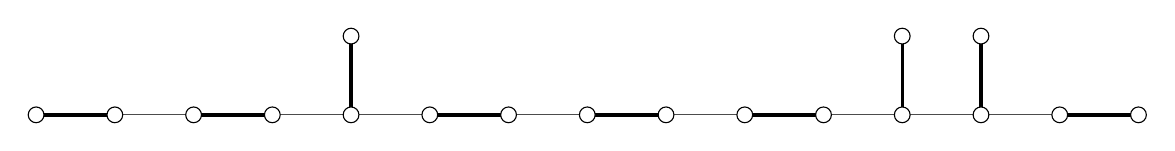
\begin{tikzpicture}
\draw[opacity = 0.7](0,0)--(14,0); \foreach\i in{4,11,12}{\draw(\i,0)--(\i,1);}
\foreach\i in{4,11,12}{\draw[very thick](\i,0)--(\i,1);} \foreach\i in{0,2,5,7,9,13}{\draw[very thick](\i,0)--(\i+1,0);}
\foreach\i in{0,1,...,14}{\draw[fill=white](\i,0)circle(0.1);} \foreach\i in{4,11,12}{\draw[fill=white](\i,1)circle(0.1);}

\end{tikzpicture}
\caption{A caterpillar with a perfect matching (black edges form a  perfect matching).}
\label{f:catmatch}
\end{figure}



 We can now solve the SIEG for caterpillars with perfect matchings. The next result is immediate from Theorem \ref{prop_zer_forc_vs_mult},  Corollary \ref{AllSimple}, and Theorem \ref{t:ZC1}.

\begin{cor}\label{c:ZCsimple} 
 Let $\GC G C$ be a coupled graph of order $2p$ such that $\MC(\GC G C)=1$.  Then  $\GC G I$ allows  a multi-set of $p$ positive  real numbers as a symplectic spectrum if and only if the elements are distinct. In particular, this applies to every 
 caterpillar  that contains a perfect matching (with  the coupling  defined by  the perfect matching).  
\end{cor}

As is the case for (standard)  zero forcing and  maximum nullity, it is possible to have the maximum symplectic multiplicity less than the coupled zero forcing number of a coupled graph.  But the situation is actually somewhat different, because for a coupled graph of order $2p$,  $\MC(\GC G C)\le p$ and $\ZC(\GC G C)\le 2p-1$ {and both bounds are sharp as illustrated by $K_{2p}$: We saw in Example \ref{random} that $\MC(K_{2p}^\PP)=p$ for any coupling, and} $\ZC(\GC {K_{2p}} C)= 2p-1$ (since $ {\ZC(\GC {K_{2p}} C)=\Zell(K_{2p})=} 2p-1$).  

%%%%%%%%%%%%%%%%%%%%%%%%%%%%%%%%%%%%%%%%%
 \section{Concluding remarks}\label{s:conclude}
In this work we have defined the ISEP-$G$ and have solved it for at least one coupling of more families of graphs than the IEP-$G$ has been solved for, with the latter involving more than a dozen authors over more than twenty years.
The following coupled graphs are symplectic spectrally arbitrary and thus the ISEP-$G$ is solved for these coupled graphs.
\bit
\item $K_{2p}^\PP$ where $\PP$ is any coupling.
\item $(K_p\du K_p)^\II$  where $\II$ pairs the vertices of one $K_p$ with the vertices of the other $K_p$.
\item $(\OL{K_p}\vee K_p)^\MM$ where $\MM$ couples each vertex of $\OL{K_p}$ with a vertex in $K_p$.
\item $K_{p,p}^\MM$  where $\MM$ couples each vertex in one partite set with a vertex in the other partite set.
\item $\tp_{2p}^\II$. 
\eit 
Other graphs for which the ISEP-$G$ is solved: 
\bit
\item All graphs of order 4  with all couplings (see Section \ref{s:order4} for details of what spectra are allowed).
\item Path $P_{2p}^\MM$ where $\MM$ is defined by the perfect matching (all eigenvalues distinct).
\item $T^\MM$ where  $T$ is a caterpillar with a perfect matching  and $\MM$ is defined by the perfect matching  (all eigenvalues distinct).
\item  $(K_p\circ K_1)^\MM$ where $\MM$  couples each leaf with its unique neighbor (any symplectic spectrum with at least two distinct symplectic eigenvalues).
\item Comb $(P_p\circ K_1)^\MM$ where $\MM$  couples each leaf with its unique neighbor (all eigenvalues distinct).
\item Sun $(C_p\circ K_1)^\MM$ where $\MM$  couples each leaf with its unique neighbor (see Corollary \ref{CpcircK1} for details of what spectra are allowed).
\item $(H\circ K_1)^\MM$ where $\MM$  couples each leaf with its unique neighbor and the IEP-$G$ is solved by specifying which ordered multiplicity lists are permitted and all spectra are allowed for these lists (depends on the spectra allowed by $H$).
\eit

These solutions have been possible through an assortment of tools we have developed for the ISEP-$G$, including the Strong Symplectic 
Spectral Property, results on symplectic positive definite matrices, and coupled zero forcing. Since labeled graphs must be used for symplectic spectra, we have introduced couplings to manage symplectically equivalent labeling, thereby substantially reducing the number of labelings that need to be considered.

 We have only begun the study of the ISEP-$G$ and many natural questions remain. 


\appendix
\section{Appendix}\label{appendix}
 This section contains the proofs of the theoretical 
properties associated with the SSSP.

\bigskip\noindent
{\bf Proof of Theorem \ref{t:verification} (SSSP Verification Matrix)}. \ms

\noi
 Recall that  $N$ is a $2p\times 2p$ positive definite matrix with labeled graph $G^L$.
Note that $\Xi(N)$ is a $(2p^2-p -|E(G)|) \times (2p^2+p)$
matrix.  Thus the equivalence of \eqref{b:verification} and \eqref{c:verification} follows from elementary linear algebra. 

Note that  
\[ 
\uvec^{-1} (\mbox{CS}( \Phi(N)))=\{ S^\top N+NS: S \in \spLA(2p)\}
,\] 
where $\mbox{CS}(\Phi(N))$  denotes the column space of
$\Phi(N)$. Also, $\uvec(\Span \SG)$  is
the subspace of $\mathbb{R}^{2p^2+p}$ consisting of those vectors 
having zero coordinate in each row of $\Phi(N)$ that 
is a row included in $\Xi(N)$.
The equivalence of \eqref{a:verification}  and \eqref{b:verification}  now follows. 
\qed\ms

The next two proofs are  essentially the same as the proofs of the Supergraph Theorem  and Bifurcation Theorem for the IEP-$G$ with the 
functions $f$  and $g$ given below  suitably modified.
 In these, we use the word ``neighborhood'' in 
the topological sense. That is, a neighborhood of a point $p$ is an open set in the pertinent topological space that contains $p$. \ms

\medskip
\noi {\bf Proof of Theorem \ref{supergraph} (Supergraph Theorem).}

\medskip
\noi
Recall  $G^L$ is a labeled graph of order $2p$,  $N\in\symp(G^L)$ has the SSSP, and   
 $H^L$ is  obtained from $G^L$ by inserting some edges.
Define the function $f \colon \spLA (2p) \times  \Span (\SG) \rightarrow \symm(2p)$
by 
\[ f(S, B)= e^{S\trans} N e^S -B.\]
Note that $f(O,O)=N$ and the linearization of $f$ at $(0,0)$
is the function $L \colon \spLA (2p) \times  \Span(G) \rightarrow \symm(2p)$ by 
\[ 
L(S,B)= N + NS + S\trans N -B.
\]
As $N$ has the SSSP, $L$ is a surjection.
As $f$ is continuous, there exists an neighborhood $U$ containing $(0,0)$ 
such that for all $(S,B) \in U$, the  $(i,j)$-entry of $f(S,B)$ is nonzero whenever
the $(i,j)$-entry of $N$ is nonzero.  By the Inverse Function theorem, there exists 
a neighborhood $V$ of $(0,0)$ contained in $U$ and a neighborhood $W$ of $N$ 
contained in $\symm(2p)$ such that $f(V)=W$.  Let $C$ be the adjacency matrix of the 
graph on $2p$ vertices whose edges are those in $H$ but not in $G$.  For $\epsilon$
sufficiently small, $N + \epsilon C \in W$.  Hence there exists $(S,B) \in V$
such that $e^{S\trans}Ne^S-B= N + \epsilon C$.  Equivalently, 
$e^{S \trans} Ne^{S} = N +B +\epsilon C$.  As $S \in \spLA (2p)$, $e^S$ is a symplectic matrix, 
and hence $e^{{S} \trans} N e^{S} $ and $N$ have the same symplectic eigenvalues.  The choice of 
$\epsilon$, $V$, $W$ and $C$ guarantee that the  labeled graph of $N + B + \epsilon C$ is $H^L$.
Therefore $e^{S{\trans}}N e^S$ is a matrix with graph $H$ and the same symplectic eigenvalues as 
$A$. 
\qed

\medskip
\noi {\bf Proof of Theorem \ref{Thm:bifurcation} (Bifurcation Theorem).}

\medskip\noi
Define the function $g\colon \spLA (2p) \times  \Span (\SG) \rightarrow \symm(2p)$
by: 
\[ g(S, B)= e^{S\trans} (N-B) e^S.\]
Note that $g(O,O)=N$ and the linearization of $g$ at $(0,0)$
is the function $L\colon \spLA (2p) \times \Span (G) \rightarrow \symm(2p)$ by 
\[ 
L(S,B)= N + NS + S\trans N -B.
\]
As $N$ has the SSSP, $L$ is a surjection.
As $g$ is continuous, there exists a neighborhood $U$ of $(0,0)$ 
such that for all $(S,B) \in U$, the  $(i,j)$-entry of $g(S,B)$ is nonzero whenever
the $(i,j)$-entry of $N$ is nonzero.  By the Inverse Function theorem, there exists 
a neighborhood $V$ of $(0,0)$ contained in $U$ and a neighborhood $W$ of $N$ 
contained in $\symm(2p)$ such that $f(V)=W$. Take $\epsilon $ small enough so that 
the $\epsilon$ ball around $N$  is contained in $W$. Suppose that $\| \widehat{N} -N \|<\epsilon$.
Then there exists $(S,B) \in V$ such that $\widehat{N}= g(S,B)= e^{S\trans} (N-B) e^{S}$.
Hence $\widehat{N}$ and $(N-B)$ have the same symplectic spectrum and $N-B$ has graph $G$. 
\qed \ms

The proof of the Matrix Liberation Lemma (Theorem \ref{liberation}) uses the {next theorem} from \cite{CS}, which needs a few definitions to present. 
 Let $U\subseteq \mathbb{R}^n$
be an open subset containing $\mathbf 0 $. 
The function $f\colon U \rightarrow \mathbb{R}^m$ is \textit{totally differentiable} 
at $\bx = \mathbf 0$ if there exists a linear transformation $d_f\colon \mathbb{R}^n \rightarrow \mathbb{R}^m $ such that
\[
\lim_{{\bx}\rightarrow \mathbf 0} \frac{ \| f(\bx)-f(\mathbf 0) -d_f\bx \|}{\|{\bx}\|}= 0. 
\]
The map $d_f$, if it exists, is unique and is called the \textit{total derivative of $f$} at ${\bx}={\bf 0}$. 

\begin{thm} {\rm \cite{CS}}
\label{IVTLiberate}
Let $f\colon\mathbb{R}^n \rightarrow  
\mathbb{R}^m$ be a smooth function
whose total derivative  $d_f$ at $\mathbf x= \mathbf 0$ exists and  let $\mathbf d= d_f(\mathbf u)$ be a nonzero vector 
in $\mbox{\rm Im}({d_f})$. 
If 
\begin{equation}
\label{cond} 
\mbox{\rm Im}(d_f) + \Span(\{ \mathbf e_i\colon i \mbox{ in support of $f(\mathbf 0)$ or the support of $\mathbf d$}\})  
= \mathbb{R}^n,
\end{equation}
then there exists $\widehat{\mathbf{x}} \in \mathbb{R}^m$
such that the support of $f(\widehat{\mathbf{x}})$ 
is the union of 
the supports of $f(\mathbf 0)$ and $\mathbf d$.  Moreover, $\widehat{\mathbf{x}}$ 
can be chosen so that the 
\begin{equation}
\label{cond'}
\mbox{\rm Im}(
d_f({\widehat{\mathbf{x}}}) + \Span(\{ \mathbf e_i \colon i \mbox{ in support of $f(\mathbf 0)$ or the support of $\mathbf d$}\})  
= \mathbb{R}^n.
\end{equation}
\end{thm} 

\medskip
\noi
{\bf Proof of Theorem \ref{liberation} (Matrix Liberation Lemma).}

\medskip\noi
{Recall that $N\in\symp(G^L)$, $R$ is a matrix in the subspace $\{ NM + M^\top N \colon M \in \spLA(2p) \}$,
and  $G^L_R$ is the labeled graph of $G^L$ in the direction of $R$.}  Assume that $N$ has the SSSP { with respect to $G^L_R$}. 
We apply Theorem \ref{IVTLiberate} to the function  
$f\colon \spLA (2p)\rightarrow \symm(2p)$
by $f(S,B)=e^{S^\top}Ne^S$,  and observe that the hypothesis 
(\ref{cond}) is equivalent to 
$\mbox{Im}(d_f)+\Span(\mathcal{S}(G_{R}))= \symm(2p)$.  \qed 

\bigskip
\noindent
{\bf Acknowledgements:} 
The authors thank the Pacific Institute for the Mathematical Sciences for partial support of H.~Gupta as a post-doctoral fellow, and the American Institute of Mathematics. 
%%%%%%%%%%%%%%%%%%%%%%%%%%%%%%%%%%%%%%%%%%%

\begin{thebibliography}{20}

\bibitem{F+13}
B.~Ahmadi, F.~Alinaghipour, M.~Cavers, S.~Fallat, K.~Meagher, and S.~Nasser. 
Minimum number of distinct eigenvalues of graphs. {\em Electron.~J.~Linear Algebra} (2013), 
26: 673-691.

\bibitem{AIM08} AIM Minimum Rank -- Special Graphs Work Group 
(F.~Barioli, W.~Barrett,  S.~Butler,   S.M.~Cioaba, D.~Cvetkovi\'c,  S.M.~Fallat,C.~Godsil,  W.~Haemers,  L.~Hogben,  R.~Mikkelson,  S.~Narayan, O.~Pryporova,   I.~Sciriha,  W.~So,   D.~Stevanovi\'c,  H.~van der Holst, K.~Vander Meulen, and A.~Wangsness).  Zero forcing sets and the minimum rank   of graphs.   {\em Lin. Alg. Appl.} 428 (2008), 
 1628--1648.

\bibitem{param}	F.~Barioli, W.~Barrett, S.~Fallat, H.T.~Hall, 
L.~Hogben, B.~Shader, P.~van den Driessche, and H.~van der Holst.  
Parameters related to tree-width, zero forcing, and maximum 
nullity of a graph.  {\em J. Graph Theory} 72 (2013),  146--177.

\bibitem{BLMNSSSY13}  
W.~Barrett,  A.~Lazenby, N.~Malloy, C.~Nelson, W.~Sexton, R.~Smith, J.~Sinckovic, and  T.~Yang. The combinatorial inverse eigenvalue problems: complete graphs and small graphs with strict inequality. {\em Electron.~J.~Linear Algebra} 26 (2013),   656--672.

\bibitem{BJ15}
R.~Bhatia and T.~Jain.
On symplectic eigenvalues of positive definite matrices.
{\it J. Math. Phys.} 56 (2015),  112201. 

\bibitem{CS} C.~Cheung and B.~Shader.
The Strong Singular Values Property. 
Under Review. \url{https://arxiv.org/abs/2507.08313}.


\bibitem{Dopico-Johnson}
F.~Dopico and
    C.R.~Johnson.
Parametrization of the matrix symplectic group and applications. \emph{SIAM J. Matrix Anal. Appl.} 31
(2009), 650--673. 

\bibitem{Zplus} J. Ekstrand, C. Erickson, H.T. Hall, D. Hay, L. Hogben, R. Johnson, N. Kingsley, S. Osborne, T. Peters, J. Roat, A. Ross, D.D. Row, N. Warnberg, and M. Young.  Positive semidefinite zero forcing. {\it{Linear Algebra Appl.}}, {\bf{439}} (2013), 1862-1874.

\bibitem{Ferg80}	W.E.~Ferguson, Jr. The construction of Jacobi and periodic Jacobi matrices with prescribed spectra. {\em Math. Comp.} 35 (1980),  1203--1220.

\bibitem{FF09}	R.~Fernandes and C.M.~da Fonseca. The Inverse Eigenvalue problem for Hermitian matrices whose graphs are cycles.  {\em Linear Multilinear Algebra} 57 (2009),  673--682.

 \bibitem{Hochstadt67a}
H.~Hochstadt. On some inverse problems in matrix theory.
{\em Arch.~Math.} 2 (1967),  201--207.

\bibitem{HLSbook} L. Hogben, J.C.-H. Lin, and B.L. Shader.  {\em Inverse Problems and Zero Forcing for Graphs}.   {Mathematical Surveys and Monographs} {270}, American Mathematical Society, Providence, RI,  2022. 

\bibitem{HJ} R.A.~Horn and C.R.~Johnson. {\em Matrix Analysis}, 2nd edition.  Cambridge University Press, Cambridge, 2013.

\bibitem{I18}
K.~D. Ikramov. On the symplectic eigenvalues of positive definite matrices.
\emph{Moscow Univ. Comput. Math. Cybernet.}  42 (2018), 1--4.

\bibitem{IMA10} IMA-ISU research group on minimum rank (M. Allison, E. Bodine, L.M. DeAlba, J. Debnath, L, DeLoss, C. Garnett, J. Grout, L. Hogben, B. Im, H. Kim, R. Nair, O. Pryporova,
K. Savage, B. Shader, and A. Wangsness Wehe). Minimum rank of skew-symmetric matrices described by a graph. {\it{Linear Algebra Appl.}} 432 (2010), 2457--2472.

\bibitem{J21}
T.~Jain. 
Sums and products of symplectic eigenvalues.
{\it Linear Algebra Appl.} 631 (2021),  67–82.



\bibitem{JLX22}
P.~Jin, Z.~Lin, and B.~Xiao.
Optimal unit triangular factorization of symplectic matrices,
{\it Linear Algebra Appl.}
650 (2022), 236--247.

\bibitem{N21}
F.~Nicacio.
Williamson theorem in classical, quantum, and statistical physics.
{\it Amer. J. Phys.} 89  (2021), 1139–1151. 

\bibitem{P22}
P.\'E. Paradan. The Horn cone associated with symplectic eigenvalues. {\it C. R. Math. Acad. Sci. Paris} 360 (2022), 1163--1168. 

\bibitem{SABT21} 
N.T.~Son, P.A.~Absil, B.~Gao, 
and T.~Stykel. Computing symplectic eigenpairs of symmetric positive-definite matrices via trace minimization and Riemannian optimization. {\it SIAM J. Matrix Anal. Appl.} 42 (2021), 1732--1757.

\bibitem{SS22} 	N.T.~Son  and T.~Stykel.   Symplectic eigenvalues of positive-semidefinite matrices and the trace minimization theorem. \emph{Elec. J. Linear Algebra} 38 (2022), 607--616.

\bibitem{W36}
J.~Williamson. On the algebraic problem concerning the normal form of linear dynamical
systems. \emph{Amer. J. Math.} 58 (1936), 141--163.


\end{thebibliography}
\end{document}



